\chapter{Continuous tempering}\label{ch:continuous-tempering}

In Chapter \ref{ch:approximate-inference} we introduced simulated tempering \citep{marinari1992simulated} as an approach for dealing with two key issues with \ac{MCMC} methods: improving exploration of multimodal distributions and allowing estimation of the normalising constant of the target distribution, which is often an important quantity for model comparison in Bayesian inference problems. Simulated tempering augments the Markov chain state with a discrete index variable controlling the \emph{inverse temperature} of the system. As the inverse temperature varies, the chain moves between exploring the typically complex target distribution at high inverse temperatures to performing updates in a simpler unimodal \emph{base distribution} at low inverse temperatures. The increased ability of the chain to move to new regions of the state space at low inverse temperatures helps improve the probability of the chain transitioning between separate modes in the target distribution. Further by computing the ratio of time spent at high and low inverse temperatures the normalising constant of the target distribution can be estimated.

Although the improved exploration of the state space and ability to estimate normalising constants offered by simulated tempering are important benefits, the algorithm can be challenging to use in practice due to sensitivity of the performance of the method to the various free parameters that need to be set. The schedule of inverse temperature values that the chain moves between must be selected, with the number of inverse temperatures chosen and their distribution across the inverse temperature range both important to getting the algorithm to perform well. More finely spaced inverse temperatures improve the ability of the chain to explore the inverse temperature space but also increase the computational demands of the method. The choice of transition operator for the updates to the inverse temperature index variable is also important, with random-walk updates tending to give a slow diffusive exploration of the inverse temperature range which can be particularly problematic when a large set of inverse temperatures is used.

It is also necessary to choose an appropriate base distribution to bridge to at low inverse temperatures, with this choice key in getting simulating tempering to perform well in high dimensional spaces. A base distribution which poorly matches the target distribution makes it unlikely the chain will mix between the low and high ends of the temperature range. Further if the volume under the target distribution (corresponding to the unknown normalising constant) differs significantly from that under the base distribution, the chain will tend to remain confined to one end of the inverse temperature range. This is typically tackled by putting prior weights on the different inverse temperature index variable values to attempt to flatten out the marginal distribution on the inverse temperatures. As appropriate values for these weights will not usually be known a-priori, generally an iterative approach is needed, with the inverse temperature distribution of initial pilot chains used to estimate the weights to use. If the mass at different inverse temperatures is very imbalanced, multiple iterations of running chains and then readjusting the weights may be required.

In the chapter we propose approaches to overcoming some of these computational issues with simulated tempering. We show how the discrete index variable used to control the inverse temperature in simulated tempering can be replaced with continuous control variable, eliminating the need to choose an appropriate number of inverse temperatures. Further the continuous nature of this auxiliary control variable means that we can apply more efficient transition operators when performing updates to the variable in the chain, including importantly in target distributions on real-valued variables allowing the control variable to be jointly updated with the target model variables with efficient \ac{HMC} transition operators. This allows the proposed approach to be easily applied in probabilistic programming frameworks such as Stan \citep{carpenter2016stan} and PyMC3 \citep{salvatier2016probabilistic} which use \ac{HMC} based inference algorithms.

We also demonstrate that a principled and effective approach for choosing appropriate base distributions for high dimensional target distributions is to fit a simple approximation to the target distribution using variational inference methods. The lower bound to the target distribution normalising constant which is maximised by variational approaches can also be used to help flatten the marginal distribution on the inverse temperatures, reducing the need for multiple iterations of pilot chains to estimate weights to flatten out the inverse temperature distribution. By using flexible parametric variational inference approaches such as \ac{ADVI} \citep{kucukelbir2016automatic}, we can fit appropriate base distributions for high-dimensional target distributions with minimal need for user intervention.

%Although \ac{HMC} is able to efficiently explore contiguous regions of high probability density in a target distribution, as with most \ac{MCMC} methods using local moves it struggles to move between isolated modes in multimodal target distributions \citep{neal2011mcmc}. Tempering methods \citep{swendsen1986replica,geyer1991markov,marinari1992simulated} which augment the state space with an temperature variable are often used to improve exploration in multimodal distributions. As the temperature variable is typically discrete however it cannot be included in \ac{HMC} updates.

%In this Chapter we present an alternative \emph{continuous tempering} approach which instead augments the state with a continuous temperature variable. This allows use of \ac{HMC} to jointly update both the temperature and original state, making the method simple to use with existing \ac{HMC} implementations. The proposed approach both improves exploration of multimodal densities and also provides estimates of the typically unknown normalising constant of the target density, which is often an important inferential quantity in its own right for model comparison \citep{gelman1998simulating}.

The work described in this chapter has previously appeared in the conference publication
\begin{itemize}
 \item Continuously tempered Hamiltonian Monte Carlo. Matthew M. Graham and Amos J. Storkey. \emph{Proceedings of the 33rd Conference on Uncertainty in Artificial Intelligence}, 2017.
\end{itemize}
I was the primary author of that publication and responsible for the contributions made in the paper, as well as performing and analysing the numerical experiments described in the paper, which are reproduced in this chapter in Section \ref{sec:ct-experiments}.

\section{Problem notation}

As in the previous chapters, our goal is to be able estimate the integrals on high-dimensional spaces which arise when performing inference in probabilistic models. We assume in this chapter that the target distribution of interest $\tgtprob$, is specified by an {unnormalised} density function $\utgtdens : \set{X} \to [0,\infty)$ defined on a real-valued space $\set{X} = \reals^D$ with respect to the Lebesgue measure. We further assume that target distribution has unbounded support on $\set{X}$ - this is non-restrictive as distributions with bounded support can typically be transformed to distributions with unbounded support using a suitable bijective map and the change of variables formula \eqref{eq:change-of-variables-discrete-bijective}.

The unnormalised density function $\utgtdens$ can be related to an energy function $\phi : \set{X} \to \reals$ by $\phi(\vct{x}) = -\log\utgtdens(\vct{x}) ~~\forall \vct{x} \in \set{X}$. The normalising constant $\normconst$ of the target density is then defined as
\begin{equation}
  \normconst = \int_{\set{X}} \exp\lpa -\phi(\vct{x})\rpa \,\dr\vct{x}.
\end{equation}
In the chapter we will consider methods both for estimating expectations with respect the target distribution and estimating the normalising constant $\normconst$, which for target distributions corresponding to the posterior distribution in a Bayesian inference problem, will correspond to the model evidence term or marginal likelihood.

We will briefly reintroduce the notation and terminology we used to describe simulated tempering in Section \ref{subsec:simulated-tempering} in Chapter \ref{ch:approximate-inference}. An ordered sequence of \emph{inverse temperatures} $\lbr \beta \rbr_{k=0}^K$ are chosen such that
\begin{equation}\label{eq:inverse-temperature-ordered-sequence}
  0 = \beta_0 < \beta_1 < \beta_2 < \dots < \beta_{K-1} < \beta_K = 1.
\end{equation}
A discrete auxiliary \emph{temperature index} variable $\rvar{k} \in \fset{1 \dots K}$ is introduce in addition to the vector of \emph{target variables} $\rvct{x} \in \set{X}$. The joint density on $\rvar{k}$ and $\rvct{x}$ is then defined as
\begin{equation}\label{eq:simulated-tempering-joint-target-density-ct}
  \pden{\rvct{x},\rvar{k}}(\vct{x},k) = \frac{1}{C}
  \exp\lpa - \beta_k \phi(\vct{x}) - (1 - \beta_k) \psi(\vct{x}) + w_k\rpa.
\end{equation}
The values $\lbrace w_k \rbrace_{k=0}^K$ are the \emph{prior weights} associated with each inverse temperature value and $\psi : \set{X} \to \reals$ defines an energy function for the \emph{base distribution} $Q$ with normalised density $q(\vct{x}) = \exp\lpa-\psi(\vct{x})\rpa$ with respect to the Lebesgue measure on $\set{X}$. Simulated tempering then constructs a Markov chain on $\set{X} \times \fset{1 \dots K}$ which has the distribution defined by the joint density \eqref{eq:simulated-tempering-joint-target-density-ct} as its unique invariant distribution, by alternating updates of the index variable $\rvar{k}$ given the target variables $\rvct{x}$ and updates of the target variables $\rvct{x}$ given the index variable $\rvar{k}$, as described in Algorithm \ref{alg:simulated-tempering}.

\section{Annealed importance sampling}\label{sec:annealed-importance-sampling}

\begin{algorithm}[!t]
\caption{Annealed importance sampling.}
\label{alg:annealed-importance-sampling}
\begin{algorithmic}
\small
    \Require
    $\phi$ : energy function corresponding to target distribution $\tgtprob$,~
    $\psi$ : energy function corresponding to base distribution $Q$,~
    $\lbrace \beta_k \rbrace_{k=0}^K$ : increasing sequence of inverse temperatures satisfying \eqref{eq:inverse-temperature-ordered-sequence},~
    $\lbrace \fwdtransop_k \rbrace_{k=0}^{K-1}$ : set of transition operators with $\transop_k$ leaving the distribution with density $\pi(\vct{x}\gvn \beta_k)$ invariant.
    \Ensure\raggedright
    $(\vct{x}_{K-1}, \ell_{K-1})$ : importance sample and log importance weight.
\end{algorithmic}
\hrule
\small
\begin{algorithmic}[1]
  \State $\vct{x}_{0} \sim Q(\cdot)$
  \State $\ell_0 \gets \beta_1 \lpa \psi(\vct{x}_0) - \phi(\vct{x}_0) \rpa$
  \For{$k \in \fset{1 \dots K-1}$}
    \State $\vct{x}_{k} \sim \transop_k(\cdot \gvn \vct{x}_{k-1})$
    \State $\ell_k \gets \ell_{k-1} + (\beta_{k+1} - \beta_{k}) \lpa \psi(\vct{x}_k) - \phi(\vct{x}_k)\rpa$
  \EndFor
  \State \Return $(\vct{x}_{K-1},\, \ell_{K-1})$
\end{algorithmic}
\end{algorithm}

An alternative approach to simulated tempering for using an ensemble of distributions corresponding to different inverse temperatures within a Monte Carlo approximate inference method, is the \ac{AIS} algorithm proposed by Neal \citep{neal2001annealed}. \ac{AIS} is a popular method in the machine learning literature for normalising constant estimation, e.g. \citep{salakhutdinov2008quantitative,wu2016quantitative}. We will briefly review the basics of the algorithm and some related methods, as we compare \ac{AIS} to our proposed approaches in the numerical experiments in Section \ref{sec:ct-experiments}.

As in simulated tempering, \ac{AIS} specifies a base distribution $Q$ on the target space $\set{X}$ with a tractable normalised density $q(\vct{x}) = \exp\lpa -\psi(\vct{x})\rpa$ and which we can tractably draw independent samples from. An increasing sequence of inverse temperatures $\lbrace \beta_k \rbrace_{k=0}^K$ defined as in \eqref{eq:inverse-temperature-ordered-sequence} are chosen, and used to define a series of distributions geometrically bridging between the densities of the base and target distributions. The distribution corresponding to an inverse temperature $\beta$ is defined as having density
\begin{equation}\label{eq:geometric-bridge-def}
  \pi(\vct{x} \gvn \beta) =
  \frac{1}{\partfunc(\beta)} \exp\lpa -\beta \phi(\vct{x}) - (1 - \beta) \psi(\vct{x}) \rpa
\end{equation}
with the inverse temperature dependent normaliser $\partfunc(\beta)$ being termed the \emph{partition function} and defined as
\begin{equation}\label{eq:partition-function-def}
  \partfunc(\beta) = 
  \int_{\set{X}} \exp\lpa -\beta \phi(\vct{x}) - (1 - \beta) \psi(\vct{x}) \rpa \,\dr\vct{x}.
\end{equation}
A sequence of $K-1$ Markov transition operator $\lbrace \fwdtransop_k \rbrace_{k=1}^{K-1}$ are defined, with the $k^{\textrm{th}}$ transition operator leaving the distribution with density $\pi(\vct{x}\gvn \beta_k)$ invariant. If $\fwdtrans_k$ is the transition density associated with the transition operator $\fwdtransop_k$ then this means that
\begin{equation}\label{eq:ais-transop-invariance}
  \pi(\vct{x}' \gvn \beta_k) = 
  \int_{\set{X}} \fwdtrans_k(\vct{x}'\gvn\vct{x})\,\pi(\vct{x}\gvn\beta_k) \,\dr\vct{x}
  \qquad \forall \vct{x}' \in \set{X}.
\end{equation}
From our discussion of Markov transition operators in Chapter \ref{ch:approximate-inference}, we know that an equivalent condition to \eqref{eq:ais-transop-invariance} is that there exists a reverse transition operator $\bwdtransop_k$ with transition density $\bwdtrans_k$ that respects the generalised balance condition
\begin{equation}\label{eq:ais-generalised-balance}
  \fwdtrans_k(\vct{x}'\gvn\vct{x})\,\pi(\vct{x} \gvn \beta_k) = 
  \bwdtrans_k(\vct{x}\gvn\vct{x}')\,\pi(\vct{x}' \gvn \beta_k)
  \quad \forall \vct{x}\in\set{X},\,\vct{x}' \in \set{X}.
\end{equation}

\ac{AIS} draws an initial state $\vct{x}_0$ from the base distribution $Q$ and sequentially applies the transition operators to generate a sequence of states, for each $k \in \fset{1 \dots K-1}$ generating a state $\vct{x}_k$ by applying the transition operator $\fwdtransop_k$ to the previous state $\vct{x}_{k-1}$, i.e. $\vct{x}_k \sim \fwdtransop(\cdot \gvn \vct{x}_{k-1})$. The sequence of $K$ generated states $\lbrace \vct{x}_k \rbrace_{k=0}^{K-1}$ forms a sample from a joint distribution with {normalised} density
\begin{equation}
  \bar{q}(\vct{x}_0,\,\vct{x}_1,\,\dots\,,\vct{x}_{K-1}) =
  q(\vct{x}_0) \prod_{k=1}^{K-1} \fwdtrans_k(\vct{x}_k\gvn\vct{x}_{k-1}).
\end{equation}
We could also consider an analogous process which draws an initial state $\vct{x}_K$ from the target distribution $\tgtprob$ and then sequentially applies the reverse transition operators, for each $k \in \fset{K-1 \dots 1}$ generating a state $\vct{x}_{k-1}$ by applying the reverse transition operator $\bwdtransop_k$ to the state $\vct{x}_{k}$, i.e. $\vct{x}_{k-1} \sim \bwdtransop(\cdot \gvn \vct{x}_{k})$. The sequence of states generated by this reverse process would have a distribution with {unnormalised} density
\begin{equation}
  \bar{p}(\vct{x}_0,\,\vct{x}_1,\,\dots\,,\vct{x}_K) =
  \utgtdens(\vct{x}_K) \prod_{k=1}^K \bwdtrans_k(\vct{x}_{k-1}\gvn\vct{x}_{k}),
\end{equation}
and a normalising constant equal to $\normconst$, i.e. equal that of the target distribution. This reverse sequence will be in general intractable to generate as we cannot draw independent samples from the target distribution. However if we consider a state sequence $\lbrace \vct{x}_k \rbrace_{k=0}^{K-1}$ generated using the forward process as a sample from an importance sampling proposal distribution with density $\bar{q}$ for the distribution defined by the reverse process with density $\bar{p}$, we have that the corresponding importance weight formed by the ratio of these two densities is
\begin{align}\label{eq:ais-importance-weight-deriv-1}
  \rharp{w}\lpa\vct{x}_0,\,\vct{x}_1,\,\dots\,,\vct{x}_{K-1}\rpa &=
  \frac
  {\bar{p}(\vct{x}_0,\,\vct{x}_1,\,\dots\,,\vct{x}_{K-1})}
  {\bar{q}(\vct{x}_0,\,\vct{x}_1,\,\dots\,,\vct{x}_{K-1})}\\
  &=
  \frac{\utgtdens(\vct{x}_{K-1})}{q(\vct{x}_0)} \prod_{k=1}^{K-1} \frac{\bwdtrans_k(\vct{x}_{k-1}\gvn\vct{x}_{k})}{\fwdtrans_k(\vct{x}_k\gvn\vct{x}_{k-1})}\\
  &=
  \frac{\utgtdens(\vct{x}_{K-1})}{q(\vct{x}_0)} \prod_{k=1}^{K-1} \frac{\pi(\vct{x}_{k-1}\gvn \beta_k)}{\pi(\vct{x}_k\gvn\beta_k)}
\end{align}
with the last line resulting from the condition that \eqref{eq:ais-generalised-balance} holds.

We can evaluate the value of this importance weight as it only involves functions we can compute (with the partition function terms $\partfunc(\beta_k)$ in the product of ratios cancelling). In particular using the definition \eqref{eq:geometric-bridge-def} in the log domain it can be shown to be equal to
\begin{equation}\label{eq:ais-log-importance-weight}
  \log \rharp{w}\lpa\vct{x}_0,\,\vct{x}_1,\,\dots\,,\vct{x}_{K-1}\rpa
  =
  \sum_{k=0}^{K-1} \lpa \beta_{k+1} - \beta_{k} \rpa \lpa \psi(\vct{x}_k) - \phi(\vct{x}_k) \rpa.
\end{equation}
This can be sequentially computed during the forward generation process by initialising $\ell_{0} = (\beta_1 - \beta_0) \lpa \psi(\vct{x}_0) - \phi(\vct{x}_0) \rpa$ and then for each $k$ calculating $\ell_k = \ell_{k-1} + (\beta_{k+1} - \beta_{k}) \lpa \psi(\vct{x}_k) - \phi(\vct{x}_k) \rpa$. The overall \ac{AIS} algorithm, including this sequential computation of the log importance weight, is described in Algorithm \ref{alg:annealed-importance-sampling}.

By the same argument as given in the discussion of importance sampling in Chapter \ref{ch:approximate-inference}, the importance weight is an unbiased estimate of the normalising constant of $\bar{p}$, i.e. $\normconst$. Further as $\vct{x}_{K-1}$ is marginally distributed according to $\tgtprob$ under the distribution of the reverse process, the final state $\vct{x}_{K-1}$ generated from the proposal distribution in the forward process can be used as an importance sample for $\tgtprob$. By performing multiple independent runs of the \ac{AIS} algorithm, we can generate a set of importance samples and weights which we can both use to estimate expectations with respect to the target distribution $\tgtprob$ and compute unbiased estimates of the normalising constant $\normconst$.

We previously argued that importance sampling typically scales poorly to high-dimensional target distributions as mismatch between the proposal and target distributions means that few samples fall in to the target distribution typical set, leading to importance weights which vary widely in magnitude and high variance estimates of both expectations with respect to the target distribution and its normalising constant. The \ac{AIS} algorithm helps overcome these issues by using Markov transition operators to define a proposal distribution which, providing the number of inverse temperatures is high enough and the transition operators mix well, should be a good match to the target. 

In the case of $K=1$ where we have just $\beta_0 = 0$ and $\beta_1 = 1$, the \ac{AIS} algorithm reverts to the standard importance algorithm described in Chapter \ref{ch:approximate-inference} using $Q$ as the proposal distribution. For $K > 1$, the Markov transition operators will perturb the initial samples from the base distribution towards regions of high probability under the target distribution. As the number of inverse temperatures is increased, the difference between invariant distributions of the transition operators corresponding to successive inverse temperatures will become smaller. If the Markov transition operators explore the space well, then for small changes in the inverse temperature the transition operators should be able to keep the state close to equilibrium for the invariant distribution for the current inverse temperature. In general as $K \to \infty$ the final importance sample will have a distribution increasingly close to the target distribution and the importance weights will give increasingly low variance estimates of $\normconst$.

%Due to Jensen's inequality the unbiased estimate of $\normconst$ corresponds to a stochastic lower bound on $\log \normconst$ \citep{grosse2015sandwiching}.
If we were able to generate samples from the reverse process described to motivate the definition of the \ac{AIS} extended target distribution, then we could use this sampled state sequence to compute importance samp\-ling estimates with respect to the distribution defined by the forward process with density $\bar{p}$. The resulting inverted importance weight
\begin{equation}\label{eq:ais-importance-weight-inv}
  \lharp{w}\lpa\vct{x}_0,\,\vct{x}_1,\,\dots\,,\vct{x}_{K-1}\rpa =
  \frac
  {\bar{q}(\vct{x}_0,\,\vct{x}_1,\,\dots\,,\vct{x}_{K-1})}
  {\bar{p}(\vct{x}_0,\,\vct{x}_1,\,\dots\,,\vct{x}_{K-1})}
\end{equation}
would then be an unbiased estimate of $\normconst^{-1}$. The \ac{BDMC} algorithm of Grosse, Ghahramani and Adams \citep{grosse2015sandwiching} uses this idea to define a scheme for upper and lower bounding $\log Z$. Due to Jensen's inequality an unbiased estimate of $\normconst$ corresponds to a stochastic lower bound on $\log \normconst$ and an unbiased estimate of $\normconst^{-1}$ corresponds to a stochastic upper bound on $\log \normconst$, with the bounds becoming tighter on average as the number of inverse temperatures $K$ used in the \ac{AIS} runs is increased and so the variance of the estimators decreased. If we run both standard `forward' \ac{AIS} runs from base to target distributions, and also `reverse' \ac{AIS} runs from target to base distributions we can therefore stochastically upper and lower bound $\log \normconst$, and by using long \ac{AIS} runs with large $K$ we can make these bounds increasingly tight.

The key computational issue with this scheme is that generally computing an exact sample from the target distribution, as required to initialise a reverse \ac{AIS} run, will be infeasible. In \citep{grosse2015sandwiching} it is observed however, that for directed generative models with observed variables $\rvct{y}$ and latent variables $\rvct{x}$, if a synthetic data set $\vct{y}$ is generated from $\prob{\rvct{y}|\rvct{x}}$ conditioned on latent variables $\vct{z}$ sampled from the prior distribution $\prob{\rvct{x}}$, then as $(\vct{x},\vct{y})$ is an exact sample from the joint distribution $\prob{\rvct{x},\rvct{y}}$, then $\vct{x}$ will be an exact sample from the posterior distribution $\prob{\rvct{x}|\rvct{y}}$ given the synthetic data $\vct{y}$. If we perform Bayesian inference experiments with synthetic data we can therefore use this approach to estimate upper and lower bounds on the model evidence term $\pden{\rvct{y}}(\vct{y})$. We use this \ac{BDMC} approach in one of the later experiments in Section \ref{sec:ct-experiments} to bound the value of the model evidence term for a synthetic image dataset under a generative image model, using these bounds a substitute for the intractable ground truth value to assess the quality of the estimates computed using our proposed approach and the other methods we test. 

%The application of \ac{HMC} updates for the transition operators $\transop_n$ in \ac{AIS} was explored in \citep{sohl2012hamiltonian} and termed \emph{Hamiltonian \ac{AIS}}. The authors suggest using many transitions composed of a single leapfrog step and partial momentum resampling can be preferable to a smaller number of transitions using multiple leapfrog steps and full momentum resampling. 

\section{Continuous temperature approaches}

In both \ac{AIS} and simulated tempering the choices of the number and spacing of the discrete inverse temperature values are key to getting the methods to perform well in complex high dimensional distributions \citep{neal1996sampling,behrens2012tuning,betancourt2014adiabatic}. To get reasonable performance it may be necessary to do preliminary pilot runs to help identify the number of inverse temperatures to use, adding to the computational and user effort burdens of using these methods. It is natural therefore to consider whether it is possible to use a continuously varying inverse temperature variable. % to side-step the need to choose a set of values. 

\emph{Path sampling} \citep{gelman1998simulating} proposes this approach, specifically in the context of estimation of normalising constants $Z$. A \emph{path} is defined as a function parametrised by a variable $\beta \in [0,1]$ which continuously maps between the target density $\exp\lpa-\phi(\vct{x})\rpa / \normconst$  and a base density $\exp\lpa-\psi(\vct{x})\rpa$, with the geometric bridge in \eqref{eq:geometric-bridge-def} a particular example, and the one that we concentrate on here.  The main proposal in \citep{gelman1998simulating} of direct relevance here is the suggestion to construct a Markov chain which leaves invariant a joint distribution on a state $(\rvct{x},\upbeta)$ with density
\vspace{-1mm}
\begin{equation}\label{eq:path-sampling-target-density}
\pden{\rvct{x},\upbeta}(\vct{x},\beta) \propto 
\exp\lpa -\beta\phi(\vct{x}) - (1-\beta)\psi(\vct{x}) \rpa\,\rho(\beta).
\end{equation}
with $\rho(\beta)$ a prior density on the inverse temperature variable analogous to the weights $\lbrace w_n \rbrace_{n=0}^N$ in simulated tempering. The authors of \citep{gelman1998simulating} suggest that the `most natural approach' to do this is to use Metropolis or Gibbs transition operator to alternate updates of $\upbeta\gvn\rvct{x}$ and $\rvct{x}\gvn\upbeta$, with they linking this idea to simulated tempering. In of the numerical experiments a random-walk Metropolis scheme is used to perform the updates to $\upbeta$ given $\rvct{x}$.

The authors of \citep{gelman1998simulating} suggest a method to use the samples of a chain with an invariant distribution with density \eqref{eq:path-sampling-target-density} to estimate $\log \normconst$ by utilising the identity
\vspace{-1mm}
\begin{equation}\label{thermodynamic-integration-path-sampling}
\log \normconst =
\int_0^1 \int_{\set{X}}
  \frac{\pden{\rvct{x},\upbeta}(\vct{x},\beta)}{\pden{\upbeta}(\beta)}\,
  \lpa \psi(\vct{x}) - \phi(\vct{x}) \rpa
\,\dr\vct{x}\,\dr\beta.
\end{equation}
A hybrid numerical integration and Monte Carlo scheme that applies the trapezium rule on a grid specified by the sampled $\upbeta$ values is suggested to approximate this integral. As the focus is normalising constant estimation there is no discussion of how to use the sampled $\rvct{x}$ states to estimate expectations with respect to the target distribution.

%A key aspect of path sampling is the utilisation of what has been called the \emph{thermodynamic integration} identity due to its use in free energy calculations in thermodynamic settings. Using the same definitions of the geometric bridge density $\pi(\vct{x}\gvn\beta)$ \eqref{eq:geometric-bridge-def} and partition function $\partfunc(\beta)$ \eqref{eq:partition-function-def} as for \ac{AIS}, and assuming that $\int_{\set{X}} \exp\lpa -\psi(\vct{x})\rpa\,\dr\vct{x} = 1$ we have that
%\begin{align}\label{eq:thermodynamic-integration-deriv}
%  \log \normconst &= \log \frac{\partfunc(1)}{\partfunc(0)} =
%  \int_0^1 \pd{\log \partfunc(\beta)}{\beta} \,\dr\beta
%   = \int_0^1 \frac{1}{\partfunc(\beta)} \pd{\partfunc(\beta)}{\beta} \,\dr\beta\\
%  & = \int_0^1 \frac{1}{\partfunc(\beta)} 
%    \int_{\set{X}} \pd{}{\beta} \exp\lpa -\beta\phi(\vct{x}) - (1-\beta) \psi(\vct{x}) \rpa \,\dr\vct{x}\,\dr\beta\\ \label{eq:thermodynamic-integration-deriv-3}
%  & = \int_0^1 \int_{\set{X}} \frac{\exp\lpa -\beta\phi(\vct{x}) - (1-\beta) \psi(\vct{x})\rpa}{\partfunc(\beta)} \lpa \psi(\vct{x}) - \phi(\vct{x}) \rpa \,\dr\vct{x}\,\dr\beta\\
%  & = \int_0^1 \int_{\set{X}} \pi(\vct{x}\gvn\beta) \lpa \psi(\vct{x}) - \phi(\vct{x}) \rpa \,\dr\vct{x}\,\dr\beta \label{eq:thermodynamic-integration-deriv-4}
%\end{align}
%Comparing the last line to \eqref{eq:ais-log-importance-weight} we can see that the \ac{AIS} log importance weight expression can be considered as an approximation of this integral, as discussed in \citep{neal2001annealed}. The integral over the inverse temperature space is approximated using a quadrature like approach by summing over a fixed grid and the integral with respect to the target variables $\vct{x}$ estimated using a Monte Carlo scheme by drawing approximate samples from $\pi(\vct{x}\gvn\beta)$.
%
%The main proposal in \citep{gelman1998simulating}  of direct relevance here is the suggestion to construct a Markov chain which leaves invariant a joint distribution on a state $(\rvct{x},\upbeta)$ with density 
%\begin{equation}\label{eq:path-sampling-target-density}
%\pden{\rvct{x},\upbeta}(\vct{x},\beta) \propto 
%\exp\lpa -\beta\phi(\vct{x}) - (1-\beta)\psi(\vct{x}) \rpa\,\rho(\beta).
%\end{equation}
%with $\rho(\beta)$ a specified prior density on the inverse temperature variable analogous to the weights $\lbrace w_n \rbrace_{n=0}^N$ in simulated tempering. The authors of \citep{gelman1998simulating} suggest that the `most natural approach' to do this is to use Metropolis or Gibbs transition operator to alternate updates of $\upbeta\gvn\rvct{x}$ and $\rvct{x}\gvn\upbeta$, with they linking this idea to simulated tempering, applying a random-walk Metropolis scheme to update $\upbeta$ given $\rvct{x}$ in one of their experiments. As $\pden{\vct{x}\gvn\beta}(\vct{x}|\beta) = \pi(\vct{x}\gvn\beta)$, by using the \eqref{eq:thermodynamic-integration-deriv-4} we have that
%\begin{equation}\label{thermodynamic-integration-path-sampling}
%\log \normconst =
%\int_0^1 \int_{\set{X}}
%  \frac{\pden{\rvct{x},\upbeta}(\vct{x},\beta)}{\pden{\upbeta}(\beta)}\,
%  \lpa \psi(\vct{x}) - \phi(\vct{x}) \rpa
%\,\dr\vct{x}\,\dr\beta.
%\end{equation}
%The authors of \citep{gelman1998simulating} suggest a method to use the samples of a chain with an invariant distribution with density \eqref{eq:path-sampling-target-density} to estimate $\log \normconst$ using a hybrid numerical integration scheme that applies a trapezium rule like algorithm on a grid specified by the sampled $\upbeta$ values. As the focus is normalising constant estimation there is no discussion of using the sampled $\rvct{x}$ states to estimate expectations with respect to the target distribution.

\emph{Adiabatic Monte Carlo} \citep{betancourt2014adiabatic} also proposes using a continuously varying inverse temperature variable, here specifically in the context of \ac{HMC}. The original Hamiltonian system $(\rvct{x},\,\rvct{p})$ is further augmented with a continuous inverse temperature coordinate $\upbeta \in [0,\,1]$. %Utilising the differential geometric theory of contact manifolds, 

A \emph{contact Hamiltonian} is defined on the augmented system, 
\begin{equation}\label{eq:contact-hamiltonian}
\begin{split}
  \hamiltonian_c(\vct{x},\,\vct{p},\,\beta) = \beta \phi(\vct{x}) &+ ( 1 - \beta ) \psi(\vct{x}) 
  + \frac{1}{2}\vct{p}\tr\mtx{M}^{-1}\vct{p} 
  + \log \partfunc(\beta) + \hamiltonian_0
\end{split}
\end{equation}
this defining a corresponding contact Hamiltonian dynamic, 
\begin{equation}\label{eq:contact-hamiltonian-flow}
  \td{\vct{x}}{t} = \pd{\hamiltonian_c}{\vct{p}}\tr\kern-3pt,\,
  \td{\vct{p}}{t} = \pd{\hamiltonian_c}{\beta} \vct{p} -\pd{\hamiltonian_c}{\vct{x}}\tr\kern-3pt,\,
  \td{\beta}{t} = \hamiltonian_c - \pd{\hamiltonian_c}{\vct{p}}\vct{p}.
\end{equation}
The flow map of this dynamic restricted to the zero level-set of the contact Hamiltonian (which the initial state can always be arranged to lie in by appropriately choosing the arbitrary constant $\hamiltonian_0$) generates trajectories which exactly conserve the contact Hamiltonian and extended state space volume element, and correspond to the thermodynamical concept of a reversible adiabatic process. 

For a quadratic kinetic energy, $\td{\beta}{t}$ is always non-positive and so forward simulation of the contact Hamiltonian flow generates non-increa\-sing trajectories in $\beta$ (and backwards simulation generates non-decreas\-ing trajectories in $\beta$). In the ideal case this allows the inverse temperature range $[0,\,1]$ to be coherently traversed without the random-walk exploration inherent to simulated tempering.

Simulating the contact Hamiltonian flow is non-trivial in practice however: the contact Hamiltonian \eqref{eq:contact-hamiltonian} depends on the log partition function $\log \partfunc(\beta)$, the partial derivatives of which require computing expectations with respect to $\pi(\vct{x}\gvn\beta)$ which for most problems is intractable to do exactly. Moreover the contact flow can encounter meta-stabilities whereby $\td{\beta}{t}$ becomes zero and the flow halts at an intermediate $\beta$ meaning the flow no longer defines a bijection between $\beta=0$ and $\beta=1$. This can be ameliorated by regular resampling of the momenta however this potentially increases random-walk behaviour of the dynamic.

An alternative \emph{extended Hamiltonian approach} for simulating a system with a continuously varying inverse temperature was proposed in the statistical physics literature \citep{gobbo2015extended}. The inverse temperature of the system is indirectly set via an auxiliary variable, which we will term the \emph{temperature control variable} $\rvar{u} \in \reals$. This control variable is mapped to an interval $[s,\,1]$, $0 < s < 1$ via a smooth piecewise defined function $\beta : \reals \to [s,\,1]$, with the conditions that for a pair of thresholds $(\theta_1,\,\theta_2)$ with $0 < \theta_1 < \theta_2$, $\beta(u) = 1 ~\forall~ |u| \leq \theta_1$, $\beta(u) = s ~\forall~ |u| \geq \theta_2$ and $s < \beta(u) < 1 ~\forall~ \theta_1 < |u| < \theta_2$.

Unlike Adiabatic Monte Carlo, an additional momentum variable $\rvar{v}$ corresponding to $\rvar{u}$ is also introduced. Although seemingly a minor difference this simplifies the implementation of the approach significantly as the system retains a symplectic structure and can continue to be viewed within the usual Hamiltonian dynamics framework. An \emph{extended Hamiltonian} is defined on the augmented system
\begin{equation}\label{eq:extended-hamiltonian-gobbo-leimkuhler}
  \extended{\hamiltonian}(\vct{x},\,u,\,\vct{p},\,v) = 
  \beta(u) \phi(\vct{x}) + \omega(u) + \frac{1}{2} \vct{p}\tr\mtx{M}^{-1}\vct{p} + \frac{v^2}{2m}
\end{equation}
where $\omega$ is a `confining potential' on $u$ and $m$ is the mass (marginal variance) associated with $\rvar{v}$. This extended Hamiltonian is separable with respect to the extended configuration $(\rvct{x},\,\rvar{u})$ and extended momentum $(\rvct{p},\,\rvar{v})$ and so can be efficiently simulated using a standard leapfrog integrator. In \cite{gobbo2015extended} the extended Hamiltonian dynamics are integrated using a Langevin scheme without Metropolis adjustment and shown to improve mixing in several molecular dynamics problems. 

Due to the condition $\beta(u) = 1 ~\forall~ |u| < \theta_1$, the set of sampled configuration states $\rvct{x}$ which have associated $|\rvar{u}| < \theta_1$ will (assuming the dynamic is ergodic and Metropolis adjustment were used) asymptotically converge in distribution to the target, and so can be used to estimate expectations without any importance re-weighting. The $\beta$ function is required to be bounded below by a $s > 0$ in \citep{gobbo2015extended} due to the base density being bridged to being an improper uniform density on $\set{X}$. The partition function $\partfunc(\beta) \to \infty$ as $\beta \to  0$ in this case, which would imply an infinite density for regions in the extended state space where $\beta(\rvar{u}) = 0$. Even with a non-zero lower bound on $\beta$, the large variations in $\partfunc\lpa\beta(\rvar{u})\rpa$  across different $\rvar{u}$ values can lead to the dynamic poorly exploring the $\rvar{u}$ dimension. In \citep{gobbo2015extended} this issue is tackled by introducing an adaptive history-dependent biasing potential on $\rvar{u}$ to try to achieve a flat density across a bounded interval $|\rvar{u}| < \theta_2$, using for example metadynamics \citep{laio2002escaping}. The resulting non-Markovian updates bias the invariant distribution of the target state however this can be accounted for either by a re-weighting scheme \citep{bonomi2009reconstructing}, or using a vanishing adaptation.

\section{Continuous tempering}\label{sec:proposed-approach}

\begin{algorithm}[t]
\caption{Gibbs continuous tempering.}
\label{alg:gibbs-continuous-tempering}
\begin{algorithmic}
\small
    \Require
    $(\vct{x}_n, \beta_n)$ : current target variables -- inverse temperature state pair,~
    $\phi$ : energy function of target distribution,~
    $\psi$ : energy function of base distribution,~
    $\zeta$  : target distribution normalising constant estimate, ~
    $\transop$ : transition operator updating only target variables $\rvct{x}$ and leaving distribution with density in \eqref{eq:ct-joint-target-density} invariant.
    \Ensure\raggedright
    $(\vct{x}_{n+1}, \beta_{n+1})$ : new target variables -- inverse temperature state pair, ~
    $(w_{0,n+1}, w_{1,n+1})$ : new importance weight pair.
\end{algorithmic}
\hrule
\small
\begin{algorithmic}[1]
  \State $\vct{x}_{n+1} \sim \transop(\cdot \gvn \vct{x}_n,\,\beta_n)$ \Comment{Update $\rvct{x}$ given current $\upbeta$.}
  \State $\Delta \gets \phi(\vct{x}) + \log \zeta - \psi(\vct{x})$ \Comment{Calculate energy difference at new state.}
  \State $u \sim \mathcal{U}(\dot \gvn 0, 1)$ \Comment{Independently sampled new $\upbeta \gvn \rvct{x}$.}
  \If{$\Delta < 0$}
     \State $\beta_{n+1} \gets 1 + \frac{\log\lpa 1 - u + \exp(-|\Delta|) u \rpa}{|\Delta|}$
  \ElsIf{$\Delta = 0$}
     \State $\beta_{n+1} \gets u$
  \Else
     \State $\beta_{n+1} \gets -\frac{\log\lpa 1 - u + \exp(-|\Delta|) u \rpa}{|\Delta|}$
  \EndIf
  \State $w_{0,n+1} \gets \frac{-\Delta}{\exp(-\Delta) - 1}$ \Comment{Calculate target distribution importance weight.}
  \State $w_{1,n+1} \gets \frac{\Delta}{\exp(\Delta) -1}$ \Comment{Calculate base distribution importance weight.}
  \State \Return $(\vct{x}_{n+1},\,\beta_{n+1})$, $(w_{0,n+1},w_{1,n+1})$
\end{algorithmic}
\end{algorithm}

We now describe our proposed continuous tempering approach. The two methods we suggest combine aspects of several of the existing algorithms we have reviewed, in particular we utilising ideas from \emph{Rao--Blackwellised tempered sampling} \citep{carlson2016partition} described in Section \ref{subsec:simulated-tempering} in Chapter \ref{ch:approximate-inference}, \emph{path sampling} \citep{gelman1998simulating} and the \emph{extended Hamiltonian} approach of \citep{gobbo2015extended}. One of the key motivations of our approaches is to minimise the number of free parameters requiring tuning by the user as far as possible.

We define a joint density on an augmented state consisting of the target variable $\rvct{x} \in \set{X}$ and an inverse temperature variable $\upbeta \in [0,1]$
\begin{equation}
\label{eq:ct-joint-target-density}
\pden{\rvct{x},\upbeta}(\vct{x},\beta) =
\frac{1}{C} \exp\lpa -\beta\phi(\vct{x}) -\beta\log\zeta -(1-\beta)\psi(\vct{x})\rpa.
\end{equation}
As previously $\phi$ and $\psi$ are the energy functions of the target and base distributions. The term $\zeta$ sets a simple prior on the inverse temperature variable and is intended to help balance the marginal densities $\pden{\upbeta}(0)$ and $\pden{\upbeta}(1)$. It should ideally be set as close to $Z$ as possible - we will motivate this in the next section.% and also discuss methods for computing reasonable approximations to use.

Importantly the conditional density on $\upbeta$ given $\rvct{x}$ corresponding to this joint density has a tractable normalised form
\begin{equation}\label{eq:ct-beta-gvn-x-density}
\pden{\upbeta|\rvct{x}}(\beta \gvn\vct{x}) = 
\frac{\exp\lpa - \beta\Delta(\vct{x})\rpa\Delta(\vct{x})}{1 - \exp\lpa-\Delta(\vct{x})\rpa},
\end{equation}
with $\Delta(\vct{x}) = \phi(\vct{x}) + \log\zeta - \psi(\vct{x})$. For $\Delta(\vct{x}) > 0$ this corresponds to an exponential distribution with rate parameter $\Delta(\vct{x})$ truncated to $[0, 1]$.   We can efficiently generate independent samples from this distribution and so an obvious method of constructing a Markov chain on the joint space is to alternate Gibbs sampling steps where new values for $\upbeta$ are independently sampled from the conditional distribution $\prob{\upbeta|\rvct{x}}$ with updates to the target variables $\rvct{x}$ with the inverse temperature $\upbeta$ fixed, for example using a Hamiltonian Monte Carlo or slice sampling transition operator. We term this approach \emph{Gibbs continuous tempering} and describe the method, including an approach for generating independent samples from the conditional distribution $\prob{\upbeta|\rvct{x}}$ in Algorithm \ref{alg:gibbs-continuous-tempering}. We will discuss the details and motivation for the additional values calculated by the algorithm shortly.

Instead of alternating separate updates of the inverse temperature $\upbeta$ and target variables $\rvct{x}$, with a continuous inverse temperature it is natural to consider jointly updating $\rvct{x}$ and $\upbeta$. In general it is easier to define transition operators on densities with unbounded support so we first define a reparameterisation of the joint target density \eqref{eq:ct-joint-target-density} using a \emph{temperature control variable} $\rvar{u} \in \reals$ related to $\upbeta$ by a standard logistic sigmoid transformation
\begin{equation}\label{eq:temperature-control-function-sigmoid}
  \upbeta = \frac{1}{1 + \exp(-\rvar{u})} = \sigma(\rvar{u})
  \iff
  \rvar{u} = \log \frac{\upbeta}{1-\upbeta}.
\end{equation}
Under this bijective transformation we can use the change of variables formula \eqref{eq:change-of-variables-vector-bijective} to define the joint density on $\rvar{u}$ and $\rvct{x}$ as
\begin{align}\label{eq:ct-joint-target-density-u}
&\pden{\rvct{x},\rvar{u}}(\vct{x},u) = \,\\ \nonumber
&\qquad\frac{\sigma(u)\lpa 1 - \sigma(u)\rpa}{C}
\exp\lpa
  -\sigma(u)\lpa \phi(\vct{x}) + \log\zeta\rpa - \lpa 1 - \sigma(u)\rpa\psi(\vct{x})
\rpa.
\end{align}
If the energy functions of the target and base distributions are differentiable, then this target density function is also differentiable with respect to all inputs and has unbounded support on $\reals^{D+1}$. In this case an obvious choice of transition operator to use is a \ac{HMC} approach.%, for example the basic \ac{HMC} transition described in Algorithm \ref{alg:hamiltonian-monte-carlo}. 

A Hamiltonian for the extended state $(\rvct{x},\,\rvar{u})$ is constructed by augmenting with associated momenta variables $(\rvct{p},\,\rvar{v})$ and then defining
\begin{align}\nonumber
  \extended{\hamiltonian}(\vct{x},u,\vct{p},v) =&
  \sigma(u) \lpa \phi(\vct{x}) + \log\zeta\rpa + 
  \lpa 1 - \sigma(u) \rpa \psi(\vct{x}) \\ \label{eq:cthmc-hamiltonian}
  &- \log\sigma(u) - \log\lpa 1- \sigma(u)\rpa +
  \frac{1}{2} \vct{p}\tr\mtx{M}^{-1}\vct{p} + \frac{v^2}{2m}.
\end{align}
As with the approach of \citep{gobbo2015extended}, this Hamiltonian is separable and the corresponding dynamic can be efficiently simulated with a leapfrog integrator. The reversible and volume-preserving simulated dynamic can then be used as a proposal generating mechanism on the joint space $(\rvct{x},\,\rvar{u},\,\rvct{p},\,\rvar{v})$ for a Metropolis--Hastings step as in standard \ac{HMC} transition described in Algorithm \ref{alg:hamiltonian-monte-carlo}. We term the approach of running \ac{HMC} in the extended joint space \emph{continuously tempered Hamiltonian Monte Carlo}. An outline of the method is given in Algorithm \ref{alg:continuously-tempered-hamiltonian-monte-carlo}; as with the previous Gibbs continuous tempering algorithm this contains steps for calculation of additional values which we will motivate shortly.

Importantly we can also equally apply more efficient adaptive \ac{HMC} variants such as the \ac{NUTS} algorithm \citep{hoffman2014no} which dynamically set the number of integration steps. In particular we can easily define models with the augmented density \eqref{eq:ct-joint-target-density-u} in probabilistic programming frameworks such as Stan and PyMC3 and exploit their efficient in-built \ac{NUTS} based inference algorithms and automatic differentiation capabilities.

\begin{algorithm}[t]
\caption[Continuously tempered \acs{HMC}.]{Continuously tempered Hamiltonian Monte Carlo.}
\label{alg:continuously-tempered-hamiltonian-monte-carlo}
\begin{algorithmic}
\small
    \Require
    $(\vct{x}_n, u_n)$ : current target variables -- temperature control state pair,\\
    $\phi$ : energy function of target distribution,~
    $\psi$ : energy function of base distribution,~
    $\zeta$  : target distribution normalising constant estimate, \\
    $\transop_{\textsc{hmc}}$ : \ac{HMC} transition operator as described in Algorithm \ref{alg:hamiltonian-monte-carlo} using Hamiltonian defined in \eqref{eq:cthmc-hamiltonian}.
    \Ensure\raggedright
    $(\vct{x}_{n+1}, u_{n+1})$ : new target variables -- temperature control state pair, ~
    $(w_{0,n+1}, w_{1,n+1})$ : new importance weight pair.
\end{algorithmic}
\hrule
\small
\begin{algorithmic}[1]
  \State $\vct{x}_{n+1}, u_{n+1} \sim \transop_{\textsc{hmc}}(\cdot \gvn \vct{x}_n,\,u_n)$ \Comment{Jointly update $(\rvct{x},\upbeta)$ using \ac{HMC}.}
  \State $\Delta \gets \phi(\vct{x}) + \log \zeta - \psi(\vct{x})$ \Comment{Calculate energy difference at new state.}
  \State $w_{0,n+1} \gets \frac{-\Delta}{\exp(-\Delta) - 1}$ \Comment{Calculate target distribution importance weight.}
  \State $w_{1,n+1} \gets \frac{\Delta}{\exp(\Delta) -1}$ \Comment{Calculate base distribution importance weight.}
  \State \Return $(\vct{x}_{n+1},\,u_{n+1})$, $(w_{0,n+1},w_{1,n+1})$
\end{algorithmic}
\end{algorithm}

We have so far neglected to discuss the key issue of how to use the sampled continuous tempering chain states to compute the expectations with respect to the target distribution $\tgtprob$ of interest and its normalising constant $\normconst$. As described in Chapter \ref{ch:approximate-inference}, in simulated tempering, typically expectations are estimated by computing averages over only the chain states for which $\rvar{k} = K$ corresponding to $\beta_K = 1$, as at convergence these states will be distributed according to the target distribution. Although simple to implement, we previously suggested that this scheme is somewhat wasteful as it means only a small proportion of generated states are used to compute estimates and this issue becomes worse as the number of inverse temperatures is increased as fewer and fewer states will corresponding to $\rvar{k} = K$.

As the inverse temperature $\upbeta$ (or equivalently temperature control variable $\rvar{u}$) is continuous in our case, there seems to potentially be even more of a problem as the probability of chains generating states with a corresponding $\upbeta$ exactly equal to one will be zero: the regions of the state space for which $\upbeta=1$ is zero-measure under the joint distribution $\prob{\rvct{x},\upbeta}$. We could form an approximate scheme by using states with $\upbeta$ values within some small tolerance of one (analogous to an \ac{ABC} approach); this would however introduce bias into the results which it would be hard to characterise, and further would require tuning the choice of tolerance. Further this method would still mean only a small subset of the chains states are utilised to estimate expectations.

In the \emph{extended Hamiltonian} approach of \citep{gobbo2015extended}, this issue is overcome by using a piecewise defined inverse temperature control function $\beta(u)$ which maps an \emph{interval} $[-\theta_1,\theta_1]$ of $\rvar{u}$ values to a corresponding inverse temperature value $\beta(\rvar{u}) = 1$. As the region of space with $\rvar{u} \in [-\theta_1,\theta_1]$ has a non-zero measure this means a non-zero number of sampled states will at convergence correspond to samples from the target distribution. Although an interesting approach, this method requires tuning the choice of the width interval $\theta_1$ of $\rvar{u}$ values mapping to $\beta(\rvar{u}) = 1$. Additionally when the chain is at states with $|\rvar{u}| \leq \theta_1$ and so the corresponding inverse temperature is $\beta(\rvar{u})=1$, the chain is effectively exploring the original target distribution, which if multimodal will mean in these periods the chain will typically mix poorly. There is therefore a tension between the requirement to keep $\theta_1$ small such that the chain maximises the time spent at low and intermediate inverse temperatures to allow for improved mixing, and the need for $\theta_1$ to not made too small so that a reasonable number of sampled chain states can be used to compute expectations with respect to the target distribution. However this tradeoff is balanced in practice, the basic scheme described will also mean that only a subset of the chain states will be used in computing expectations.

In Chapter \ref{ch:approximate-inference} we discussed simulated tempering in the broader context of auxiliary variable methods where the target distribution to corresponds to a conditional distribution given a value or set of values of the auxiliary variables. We made the observation there that the standard estimator used to compute expectation in these methods was closely related to rejection sampling. We at that point suggested that alternative approaches could be considered which are instead based on importance sampling. We use that intuition here to suggest an estimator for expectations with respect to the target distribution using continuous tempering chains. The key idea is to use the marginal distribution $\prob{\rvct{x}}$ on the target variables under the joint density \eqref{eq:ct-joint-target-density} as the proposal distribution for an importance sampling estimator for expectations with respect to the target distribution. As the generated target variable states of continuous tempering chains will be, at convergence, distributed according to $\prob{\rvct{x}}$ we can use (all) the sampled $\rvct{x}$ values to estimate expectations with respect to $\prob{\rvct{x}}$.

The target distribution $\tgtprob$ is equal to $\prob{\rvct{x}|\beta}(\cdot \gvn 1)$ and so expectations with respect to $\tgtprob$ correspond to
\begin{equation}
\expc{f(\rvct{x})\gvn\upbeta=1} =
\int_{\set{X}} f(\vct{x})\,\pden{\rvct{x}|\upbeta}(\vct{x}\gvn 1)\,\dr\vct{x}.
\end{equation}
We can use an importance sampling approach to re-express this integral with respect to the conditional distribution $\prob{\rvct{x}|\upbeta}$ as expectations with respect to the the marginal distribution $\prob{\rvct{x}}$, giving the following
\begin{align}
\expc{f(\rvct{x})\gvn\upbeta=1} &=
\frac{
  \int_{\set{X}} 
    f(\vct{x})\, \frac{\pden{\rvct{x}|\upbeta}(\vct{x}\gvn 1)}{\pden{\rvct{x}}(\vct{x})} \, \pden{\rvct{x}}(\vct{x})
  \,\dr\vct{x}
}{
  \int_{\set{X}} 
    \frac{\pden{\rvct{x}|\upbeta}(\vct{x} \gvn 1)}{\pden{\rvct{x}}(\vct{x})} \, \pden{\rvct{x}}(\vct{x})
  \,\dr\vct{x}
} \\ \label{eq:ct-target-expc-reparam}
&=
\frac{
  \int_{\set{X}} 
    f(\vct{x})\, \pden{\upbeta|\rvct{x}}(1 \gvn \vct{x}) \, \pden{\rvct{x}}(\vct{x})
  \,\dr\vct{x}
}{
  \int_{\set{X}} 
    \pden{\upbeta|\rvct{x}}(1 \gvn \vct{x}) \, \pden{\rvct{x}}(\vct{x})
  \,\dr\vct{x}
} .
\end{align}
%This identity shows that we can compute expectations 
As at convergence the $\rvct{x}$ components of the chain states will be marginally distributed according to $\pden{\rvct{x}}$ we can therefore construct consistent estimators for \eqref{eq:ct-target-expc-reparam} from the sampled target variable states $\lbrace \vct{x}_n \rbrace_{n=1}^N$ of a continuous tempering chain, by computing weighted averages
\begin{equation}\label{eq:ct-target-expc-estimator}
\expc{f(\rvct{x})\gvn\upbeta=1} =
\lim_{N \to \infty}
\frac
{\sum_{n=1}^N \lpa w_1\lpa \vct{x}_n\rpa f\lpa\vct{x}_n\rpa\rpa}
{\sum_{n=1}^N\lpa w_1\lpa \vct{x}_n\rpa \rpa}.
\end{equation}
The importance weights take values according to $\pden{\upbeta|\rvct{x}}$ \eqref{eq:ct-beta-gvn-x-density}
\begin{equation}\label{eq:ct-target-expc-estimator-importance-weight}
w_1(\vct{x}) = \pden{\upbeta \rvct{x}}(1 \gvn \vct{x}) = \frac{\Delta(\vct{x})}{\exp\lpa\Delta(\vct{x})\rpa - 1}.
\end{equation}
Intuitively this estimator \eqref{eq:ct-target-expc-estimator} seems reasonable, more highly weighting sampled target variables $\vct{x}$ for which $\pden{\upbeta \rvct{x}}(1 \gvn \vct{x})$ is high. Importantly unlike the standard rejection sampling type estimator it does not depend on the actual sampled inverse temperature state values and can be validly computed even if no sampled state pair ever has $\beta = 1$ which will generally be the case for continuous tempering, and uses information from all of the chain target variable states to compute estimates.

By an analogous construction, we can also estimate expectations with respect to the base distribution $Q$, corresponding to $\prob{\rvct{x}|\upbeta}(\cdot|0)$ using
\begin{equation}\label{eq:ct-base-expc-estimator}
\expc{f(\rvct{x})\gvn\upbeta=0}
= \lim_{N \to \infty}
\frac
{\sum_{n=1}^N \lpa w_0\lpa \vct{x}_n\rpa f\lpa\vct{x}_n\rpa\rpa}
{\sum_{n=1}^N\lpa w_0\lpa \vct{x}_n\rpa \rpa}
\end{equation}
with the corresponding importance weights defined by
\begin{equation}\label{eq:ct-base-expc-estimator-importance-weight}
w_0(\vct{x}) = \pden{\upbeta \rvct{x}}(0 \gvn \vct{x}) = \frac{\Delta(\vct{x})}{1 - \exp\lpa - \Delta(\vct{x})\rpa}.
\end{equation}
Typically the base distribution will have known moments (e.g. mean and covariance of a Gaussian base distribution) which can be compared to the estimates calculated using this estimator \eqref{eq:ct-base-expc-estimator} to check for convergence problems. Convergence of the estimates to the true moments is not a sufficient condition for convergence of the chain to the distribution defined by \eqref{eq:ct-joint-target-density} but is necessary.

Although we can calculate the importance weights \eqref{eq:ct-target-expc-estimator-importance-weight} and \eqref{eq:ct-base-expc-estimator-importance-weight} in a post-processing step after running the chain, the energy difference terms $\Delta(\vct{x})$ required to compute them will typically already be computed as part of the chain state updates - for example $\Delta(\vct{x})$ is computed to independently generate a new $\upbeta$ value from $\prob{\upbeta|\rvct{x}}$ in Gibbs continuous tempering, and for continuously tempered \ac{HMC} the final Metropolis accept step will require calculating the Hamiltonian\eqref{eq:cthmc-hamiltonian} at the new state which involves evaluating $\Delta(\vct{x})$. It will therefore generally be more efficient to compute these weights as part of each update; we show such a scheme in Algorithms \ref{alg:gibbs-continuous-tempering} and \ref{alg:continuously-tempered-hamiltonian-monte-carlo}.

We can also use the importance weights to construct an estimator for the normalising constant $\normconst$ of the target density. The inverse temperature marginal density $\pden{\upbeta}$ corresponding to \eqref{eq:ct-joint-target-density} is
\begin{equation}\label{eq:ct-beta-marginal}
\pden{\upbeta}(\beta) = 
\frac{1}{C\zeta^\beta} \int_{\set{X}} 
  \exp\lpa -\beta\phi(\vct{x}) -(1-\beta) \psi(\vct{x})\rpa
\,\dr\vct{x} =
\frac{\partfunc(\beta)}{C\zeta^\beta}.
\end{equation}
We therefore have that
\begin{equation}\label{eq:ct-beta-marginal-0-1}
\pden{\upbeta}(0) = \frac{1}{C},~
\pden{\upbeta}(1) = \frac{\normconst}{C \zeta}
\implies
\normconst = \frac{\pden{\upbeta}(1)}{\pden{\upbeta}(0)} \zeta.
\end{equation}
We can use \eqref{eq:ct-beta-gvn-x-density} to write the marginal density $\pden{\upbeta}$
\begin{equation}\label{eq:ct-beta-marginal-estimator}
\pden{\upbeta}(\beta) = 
\int_{\set{X}} \pden{\upbeta|\rvct{x}}(\beta \gvn \vct{x})\, \pden{\rvct{x}}(\vct{x}) \,\dr\vct{x} =
\expc{\pden{\upbeta|\rvct{x}}(\beta \gvn \rvct{x})}
\end{equation}
and so the marginal densities of $\upbeta=0$ and $\upbeta=1$ can be written
\begin{equation}\label{eq:ct-beta-marginal-0-1-estimators}
\pden{\upbeta}(0) = \expc{w_0(\rvct{x})}
\quad\textrm{and}\quad
\pden{\upbeta}(1) = \expc{w_1(\rvct{x})}.
\end{equation}
Therefore given target variable samples $\lbr \vct{x}_n\rbr_{n=1}^N$ from a continuous tempering chain we have the following consistent estimator for $\normconst$
\begin{equation}\label{eq:ct-norm-const-estimator}
\normconst = \frac{\expc{w_1(\rvct{x})}}{\expc{w_0(\rvct{x})}} \zeta = 
\lim_{N\to\infty} \frac
{\sum_{n=1}^N\lpa w_1\lpa \vct{x}_n\rpa\rpa}
{\sum_{n=1}^N\lpa w_0\lpa \vct{x}_n\rpa\rpa}
\zeta,
\end{equation}
This can be seen to be a continuous analogue of the \emph{Rao-Blackwellised} estimator \eqref{eq:simulated-tempering-norm-const-est-rb} proposed in \cite{carlson2016partition} and discussed in Section \ref{subsec:simulated-tempering}.

\section{Choosing a base distribution}\label{sec:choosing-base-density}

We now consider criteria for selecting an appropriate base distribution $Q$ to use with tempering methods. We claimed in the introduction that the choice of base distribution was key to the performance of tempering methods in complex high-dimensional targets, with the degree of match between the base and target determining the ability of the chain to mix between low and high inverse temperatures. In this section we formalise this statement by deriving some basic properties of the logarithm of the inverse temperature marginal density $\log\pden{\upbeta}$ and its relation to the \ac{KL} divergences between $Q$ and $P$. We will then use these properties to motivate specific computational schemes for fitting a base distribution.

Taking logarithms of \eqref{eq:ct-beta-marginal} and recalling the previous definition of the geometric bridge density $\pi(\vct{x}\gvn\beta)$ \eqref{eq:geometric-bridge-def}
\begin{align} \nonumber
  \log\pden{\upbeta}(\beta) &=
  \log \int_{\set{X}} \exp\lpa - \beta\phi(\vct{x}) - (1-\beta)\psi(\vct{x})\rpa\,\dr\vct{x}
  - \log C - \beta \log \zeta
  \\ \label{eq:ct-log-beta-marginal}
  &= \log\int_{\set{X}}\pi(\vct{x}\gvn\beta)\,\dr\vct{x} - \log C - \beta\log\zeta.
\end{align}
We will first show that $\log\pden{\upbeta}$ is convex. Differentiating \eqref{eq:ct-log-beta-marginal} with respect to the inverse temperature and using the earlier definition of the partition function $\partfunc(\beta)$ \eqref{eq:partition-function-def} gives
\begin{align}\nonumber
  \pd{\log\pden{\upbeta}}{\beta} &=
  \int_{\set{X}} 
  \lpa \psi(\vct{x}) - \phi(\vct{x}) - \log\zeta \rpa
  \frac{\exp\lpa - \beta\phi(\vct{x}) - (1-\beta)\psi(\vct{x})\rpa}{\partfunc(\beta)}
  \,\dr\vct{x}\\
  &=\label{eq:ct-log-beta-marginal-deriv}
  \int_{\set{X}} 
  \lpa \psi(\vct{x}) - \phi(\vct{x}) - \log\zeta \rpa \pi(\vct{x}\gvn\beta)
  \,\dr\vct{x}.
\end{align}
Differentiating again then gives after some manipulation
\begin{equation}\label{eq:ct-log-beta-marginal-second-deriv}
\begin{split}
  \pd{^2\log\pden{\upbeta}}{\beta^2} &=
  \int_{\set{X}} \lpa \psi(\vct{x}) - \phi(\vct{x})\rpa^2 \pi(\vct{x}\gvn\beta)\,\dr\vct{x} -
  \\&\phantom{=}\qquad
  \lpa
    \int_{\set{X}} \lpa \psi(\vct{x}) - \phi(\vct{x})\rpa\pi(\vct{x}\gvn\beta)\,\dr\vct{x}
  \rpa^2.
\end{split}
\end{equation}
As the square function is convex by Jensen's inequality we have that
\begin{equation*}
\begin{split}
  &\lpa
    \int_{\set{X}} \lpa \psi(\vct{x}) - \phi(\vct{x})\rpa\pi(\vct{x}\gvn\beta)\,\dr\vct{x}
  \rpa^2 \leq
  \int_{\set{X}} \lpa \psi(\vct{x}) - \phi(\vct{x})\rpa^2 \pi(\vct{x}\gvn\beta)\,\dr\vct{x}.
\end{split}
\end{equation*}
Therefore $\pd{^2\log\pden{\upbeta}}{\beta^2} \geq 0$ and so $\log\pden{\upbeta}$ is convex.

We now show that gradients of $\log\pden{\upbeta}$ at the end-points $\beta=0$ and $\beta=1$ are related to the \ac{KL} divergences between the base and target distributions. We first recall the definition of the \ac{KL} divergence between two probability distributions $P$ and $Q$ on a space $\set{X}$ with $P$ absolutely continuous with respect to $Q$ as
\begin{equation}\label{eq:kullback-leibler-probability-measures-ct}
  \kldiv{P}{Q} =
  \int_{\set{X}} \log\lpa\td{P}{Q}\rpa \,\dr P,
\end{equation}
which is read as the \ac{KL} divergence from $P$ to $Q$. For distributions $P$ and $Q$ on a real-valued space $\set{X} = \reals^D$ defined by densities $p$ and $q$ with respect to the Lebesgue measure we further have that
\begin{equation}\label{eq:kullback-leibler-probability-densities-ct}
  \kldiv{P}{Q} = \kldiv[\lambda]{p}{q} =
  \int_{\set{X}} p(\vct{x}) \, \log\frac{p(\vct{x})}{q(\vct{x})} \, \dr\vct{x}.
\end{equation}
Considering first the value of $\pd{\log\pden{\upbeta}}{\beta}$ at the upper end point $\beta=1$
\begin{align}
  \pd{\log\pden{\upbeta}}{\beta}(1) &= 
  \int_{\set{X}} 
  \lpa \psi(\vct{x}) - \phi(\vct{x}) - \log\zeta \rpa \frac{1}{Z}\exp\lpa-\phi(\vct{x})\rpa
  \,\dr\vct{x}\\
  &=
  \int_{\set{X}}
  \lpa -\log q(\vct{x}) +\log \tgtdens(\vct{x}) +\log Z - \log\zeta \rpa
  \tgtdens(\vct{x})
  \,\dr\vct{x}\\
  &=
  \int_{\set{X}} 
    \log\frac{\tgtdens(\vct{x})}{q(\vct{x})} \tgtdens(\vct{x}) 
  \,\dr\vct{x} + \log Z - \log\zeta \\
  &=
  \kldiv{\tgtprob}{Q} + \log Z - \log\zeta.
\end{align}
Equivalently for the lower end point $\beta=0$
\begin{align}
  \pd{\log\pden{\upbeta}}{\beta}(0) &= 
  \int_{\set{X}} 
  \lpa \psi(\vct{x}) - \phi(\vct{x}) - \log\zeta \rpa \exp\lpa-\psi(\vct{x})\rpa
  \,\dr\vct{x}\\
  &=
  \int_{\set{X}}
  \lpa -\log q(\vct{x}) +\log \tgtdens(\vct{x}) +\log Z - \log\zeta \rpa
  q(\vct{x})
  \,\dr\vct{x}\\
  &=
  -\int_{\set{X}} 
    \log\frac{q(\vct{x})}{\tgtdens(\vct{x})} q(\vct{x}) 
  \,\dr\vct{x} + \log Z - \log\zeta \\
  &=
  -\kldiv{Q}{\tgtprob} + \log Z - \log\zeta.
\end{align}

The convexity of the log marginal density means that gradients of $\log\pden{\upbeta}$ at the end-points give a lot of information about the shape of the log marginal density. For the purposes of improving mixing of tempered chains across the inverse temperature range, we ideally want the marginal density on the inverse temperatures $\pden{\upbeta}$ to be as flat as possible. As $\log\pden{\upbeta}$ is convex, if we set $\log \zeta = \log Z$ and chose a base distribution $Q$ such that $\kldiv{\tgtprob}{Q} = \kldiv{Q}{\tgtprob} = 0$ we would have $\log\pden{\upbeta}$ is constant and so the marginal density would be uniform across $[0,1]$. Of course in reality we do not know $\log Z$ and $\kldiv{\tgtprob}{Q} = \kldiv{Q}{\tgtprob} = 0$ would only be satisfied if we used the target distribution as the base distribution, which would negate any benefit from using a tempering approach.

More practically we need to constrain $Q$ to be in a family of distributions amenable to exploration, such that tempered chains gain from an improved ability to move around the space when at low inverse temperatures. Under that constraint, we then ideally want the gradients of the (logarithm of the) marginal density $\pden{\upbeta}$ to be as close to zero as possible at $\beta=0$ and $\beta=1$ such that the marginal density is as flat as possible. This suggests we want to minimise $\kldiv{Q}{\tgtprob}$ or $\kldiv{Q}{\tgtprob}$ or some combination of thereof, subject to $Q$ being in a `simple' family.

This is exactly the task considered by the variational inference methods discussed in Appendix \ref{app:optimisation-based-approximate-inference}. The standard variational inference approach involves fitting an approximate distribution $Q$ in a fixed family to a target distribution $\tgtprob$ by minimising the \ac{ELBO} variational objective $\log \normconst -\kldiv{Q}{P}$ (so-called as in Bayesian inference problems $\normconst$ corresponds to the model evidence and $\kldiv{Q}{P} \geq 0$ therefore the \ac{ELBO} lower bounds the evidence). If we were to fit a base distribution $Q$ in this manner and set $\log \zeta$ to the final value of the (estimated) variational objective, the gradient of the log marginal density at $\beta=0$ should be close to zero. 

In terms of the choice of variational inference approach, in some cases we may be able to use variational methods specifically designed for the target distribution family. More generally methods such as \ac{ADVI} \citep{kucukelbir2016automatic} provide a black-box framework for fitting variational approximations to differentiable target densities. In models such as \ac{VAE} \citep{kingma2013auto,rezende2014stochastic} a parametric variational approximation to the target density of interest (e.g. posterior on latent space) is fitted during training of the original model, in which case it provides a natural choice for the base distribution as observed in \citep{wu2016quantitative}. 

 %As the log marginal density $\log\pden{\upbeta}$ is convex  this will typically lead to a marginal density which is maximal at $\upbeta=1$ and monotonically decreases as $\upbeta \to 0$. Depending on how close the base distribution can be made to the target and so the gradient at $\upbeta$

A potential problem with this approach is that the classes of target distribution that we are particularly interested in applying our approach to --- those with multiple isolated modes --- are precisely the same distributions that simple variational approximations will tend to fit poorly, the divergence $\kldiv{Q}{\tgtprob}$ being minimised favouring `mode-seeking' solutions which usually fit only one mode well as illustrated in \ref{fig:variational-objective-comparison} in Appendix \ref{app:optimisation-based-approximate-inference}. This both limits how small the divergence from the base to target can be made, but also crucially is undesirable as we wish to use the base distribution to move between modes in the target.

One option would be to instead to minimise the reversed \ac{KL} divergence $\kldiv{\tgtprob}{Q}$, this tending to produce `mode-covering' solutions that match global moments. Methods such as \acf{EP} \citep{minka2001expectation} do allow moment-matching approximations to be found and \ac{EP} methods may be a good option in the cases were they are applicable to the distribution of interest . Another possibility would be to use an alternative divergence in a variational framework that favours mode-covering solutions, with methods using the $\chi$-divergence \citep{dieng2016chi} and R\'enyi divergence \citep{li2016renyi} having been recently proposed in this context and discussed in Section \ref{sec:variational-methods} in Appendix \ref{app:optimisation-based-approximate-inference}.

A further alternative is to fit multiple local variational approximations $\lbrace q_i(\vct{x}) \rbrace_{i=1}^L$ by minimising the \ac{ELBO} variational objective from multiple random parameter initialisations (discarding any duplicate solutions as measured by some distance tolerance between the variational parameters), each approximating a single mode well. We can then combine these local approximations into a global approximation $q(\vct{x})$, for example using a mixture model
\begin{equation}\label{eq:variational-mixture-approx}\textstyle
  m(\vct{x}) = \frac{1}{\zeta} \sum_{i=1}^L \lpa \exp(\ell_i) q_i(\vct{x}) \rpa,~~
  \zeta = \sum_{i=1}^L \exp(\ell_i),
\end{equation}
with $\ell_i$ the final variational objective value for $q_i$. If the local approximations had non-overlapping support this would lead to a global approximation which is guaranteed to be at least as close in \ac{KL} divergence as any of the local approximations and a $\log \zeta$ which is at least as tight a lower bound on $\log Z$ as any of the individual $\ell_i$ \citep{zobay2009mean}. Often we may wish to use local approximations with overlapping support (e.g. Gaussian) where the guarantee does not apply. However for the cases of target distributions with multiple isolated modes the `overlap' (regions with high density under multiple $q_i$) between local Gaussian approximations to each mode will often be minimal and so the method is still a useful heuristic. A mixture distribution is unlikely to itself be a good choice of base distribution however, as it will tend to be multimodal. We can therefore instead use a base distribution with moments matched to the fitted mixture, e.g. $q(\vct{x}) = \nrm{\vct{x}\gvn\vct{\mu},\mtx{\Sigma}}$ with mean and covariance matched to the mean and covariance of the mixture $m(\vct{x})$.

For complex target distributions typically even with a variational fitting approach, the \ac{KL} divergences between base and target distributions will remain relatively large. For approaches based on minimising $\kldiv{Q}{P}$ and setting $\log \zeta$ to the final variational objective, then as $\log \zeta$ will be a lower bound on $\log Z$ the as result of \eqref{eq:ct-beta-marginal-0-1} in this case we will have $\pden{\upbeta}(1) \geq \pden{\upbeta}(0)$ (this can also be seen from the convexity of the log marginal density and that the log marginal density gradient at $\beta=0$ should be approximately zero), with the degree of discrepancy depending on the divergence between the base and target distributions. If the divergence remains large, in this case tempered chains will tend to remain at inverse temperatures close to one, limiting the gain from the temperature augmentation. Equally if an approach is used which gives $\log\normconst <  \log\zeta$ and so $\pden{\upbeta}(1) < \pden{\upbeta}(0)$ then if the discrepancy is large tempered chains will tend to remain confined to low inverse temperatures, and the variance of the estimator \eqref{eq:ct-target-expc-estimator} will become high as performance will be similar to using the base distribution $Q$ directly in a simple importance sampling estimator (without the benefit of drawing independent samples).

%If the \ac{KL} divergence from the base to target distribution is high, the bounds on the marginal in \eqref{eq:partition-function-bounds} become increasingly loose and this tends to lead to low densities on intermediate inverse temperatures. This reduces the ability of the \ac{MCMC} dynamic to move between the inverse temperatures corresponding to the target and base distributions and so the mixing gain from the augmentation. Similarly from \eqref{eq:beta-marginal-0-1} the density ratio $\pden{\upbeta}(1) \,/ \pden{\upbeta}(0)$ is $\exp(\log \normconst - \log \zeta)$, and so for large $|\log\normconst - \log\zeta|$ the dynamic will tend to spend most of the time close to $\upbeta = 1$ if $\log \normconst  > \log \zeta$ or $\upbeta = 0$ if $\log \normconst < \log \zeta$. In the former case there will be limited gain from using the extended space while in the latter the variance of the estimator in \eqref{eq:ct-target-expc-estimator} will be comparable to using an importance sampling estimator for the target using samples from the base distribution.

A natural approach to try to ameliorate these effects is to use an iterative method analogous to the approaches often used in \ac{ST} to choose the prior weights on the inverse temperatures \citep{geyer1995annealing,carlson2016partition}. An initial $Q$ and $\log \zeta$ are chosen for example using a Gaussian variational approximation to the target distribution as described above. An initial pilot tempered chain is then run. The sampled states from this chain can then be used to both compute an estimate for $\log \normconst$ using \eqref{eq:ct-norm-const-estimator} and updated estimates of the target density mean and covariance using \eqref{eq:ct-target-expc-estimator}. A new Gaussian base distribution $Q$ can then be specified with the updated mean and covariance estimates and $\log \zeta$ chosen to be the updated $\log \normconst$ estimate. Samples of the new joint density can then be used to update $\log \zeta$ and $Q$ again and so on. Although this adds significantly to the computational and user effort burden, the use of an initial variational approach can potentially reduce the amount of iteration used significantly compared to using a simple non-informative base distribution such as the prior distribution of a posterior target distribution.

%This is analogous to the iterative approaches often used in \ac{ST} to choose the prior weights on the inverse temperatures \citep{geyer1995annealing,carlson2016partition}. 

A difficulty presented by the use of a continuous inverse temperature formulation is that it is not as trivial as the discrete case to attempt to flatten out the overall marginal distribution on the inverse temperature by using estimates from an initial run of the relative probabilities (densities) of intermediate $\upbeta \in (0, 1)$ (with the $\log \zeta$ value controlling the relative densities of $\upbeta = 1$ and $\upbeta = 0$). While in the discrete case the weights $\lbrace w_n \rbrace_{n=0}^N$ can be used to arbitrarily reweight the marginal $\prob{\upbeta = \beta_n}$, in the continuous case a suitably expressive parametric family across the interval $[0,\,1]$ would need to be chosen for the prior density. We do not investigate this issue further here but it could form an important line of future developments of the algorithm.%This can be achieved by using a cubic spline for $\rho(\beta)$ fitted to the inverse of the estimated marginal densities at a series of points, with the resulting piecewise defined exponentially weighted cubic having a tractable integral.

\section{Numerical experiments}\label{sec:ct-experiments}

%We performed a series of numerical experiments to evaluate the performance of the proposed continuous tempering approaches compared to existing methods.
We now move on to discussing the results of three numerical experiments comparing the proposed continuous tempering approaches to simulated tempering and \ac{AIS}.

%\subsection{One-dimensional bimodal target}\label{subsec:exp-bimodal-target}
%
%\begin{figure}[!t]
%\begin{subfigure}[b]{.8\linewidth}
%\vskip 0pt
%\centering
%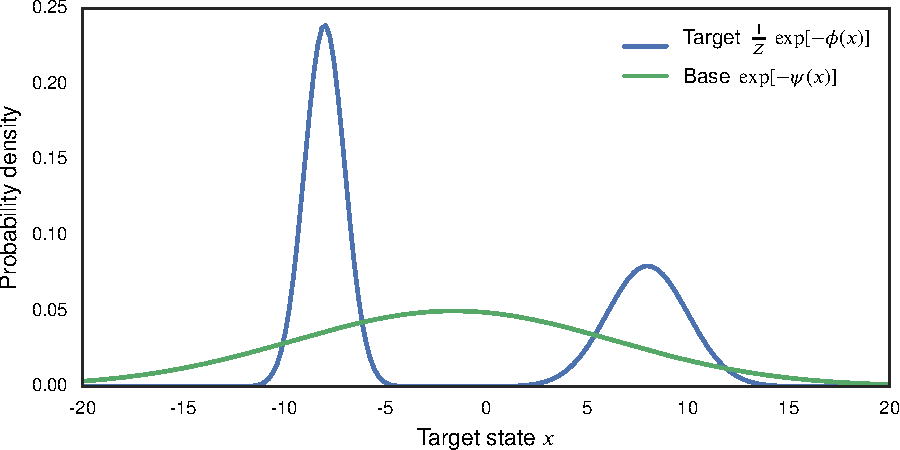
\includegraphics[width=0.95\textwidth]{images/continuous-tempering/bimodal-gm-target-and-gaussian-base} 
%\caption{Target (blue curve) \& base (green curve) density functions.}\label{sfig:bimodal-gm-target-and-gaussian-base}
%\end{subfigure}
%\\
%\begin{subfigure}[b]{.8\linewidth}
%\vskip 0pt
%\centering
%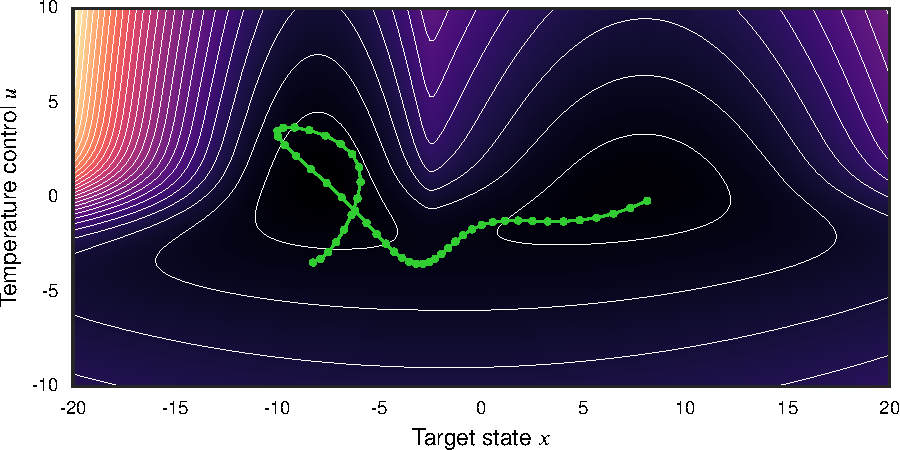
\includegraphics[width=0.95\textwidth]{images/continuous-tempering/jct-energy-and-trajectory} 
%\caption{Joint energy (contour plot) \& example trajectory (green curve).}\label{sfig:jct-energy-and-trajectory}
%\end{subfigure}%
%\\
%\begin{subfigure}[b]{.8\linewidth}
%\vskip 5pt
%\centering
%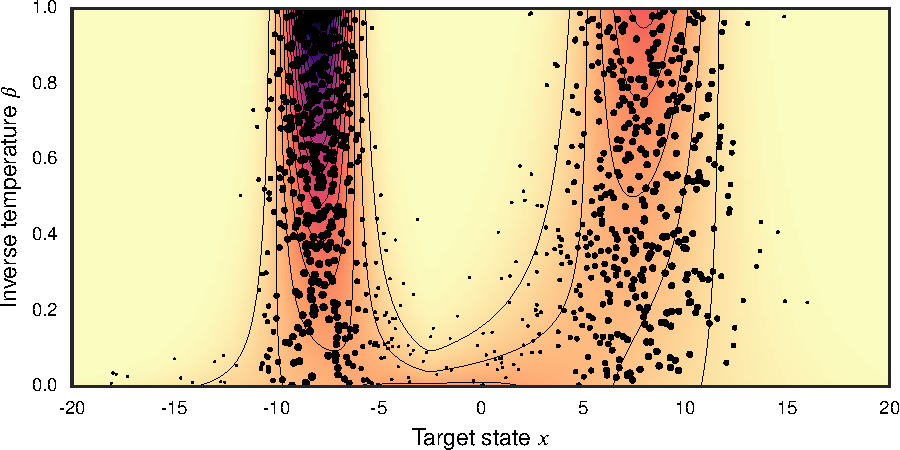
\includegraphics[width=0.95\textwidth]{images/continuous-tempering/jct-prob-dens-and-joint-samples}
%\caption{Joint density (contour plot) and \ac{CT} \ac{HMC} samples (circles).}\label{sfig:jct-prob-dens-and-joint-samples}
%\end{subfigure}
%\\
%\begin{subfigure}[b]{.8\linewidth}
%\vskip 5pt
%\centering
%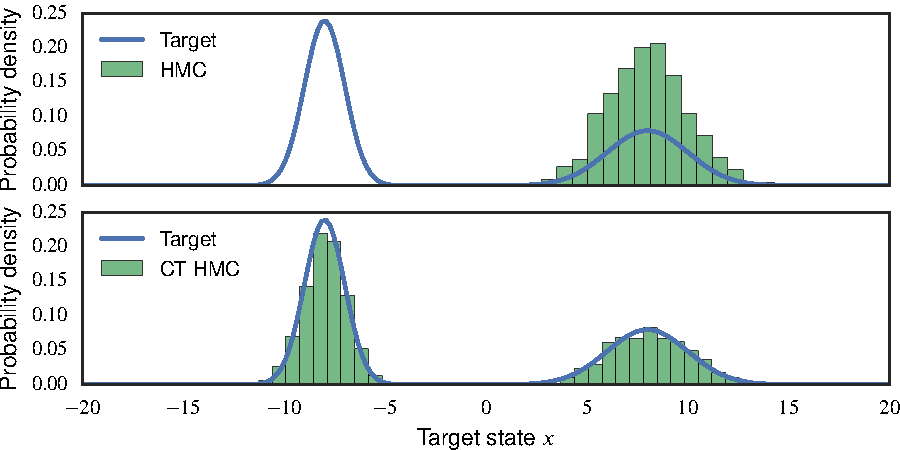
\includegraphics[width=0.95\textwidth]{images/continuous-tempering/jct-and-hmc-target-histograms}
%\caption{Histograms from \ac{HMC} (top) and \ac{CT} \ac{HMC} (bottom) samples.}\label{sfig:jct-and-hmc-target-histograms}
%\end{subfigure}
%\caption[Continuous tempering visualisations.]{Visualisations of \ac{CT} in a bimodal univariate target density. \subref{sfig:bimodal-gm-target-and-gaussian-base} A two-component Gaussian mixture target density (blue curve) and Gaussian base density (green curve) with mean and variance matched to the target. \subref{sfig:jct-energy-and-trajectory} The extended potential energy on the target state $\rvar{x}$ and temperature control variable $\rvar{u}$ (contour plot - dark colours indicate low energy) and an example simulated Hamiltonian trajectory in the joint space (green curve). The temperature control variable bridges the base and target densities lowering energy barriers in the target space. \subref{sfig:jct-prob-dens-and-joint-samples} Joint density on the target state $\rvar{x}$ and inverse temperature $\upbeta$ \eqref{eq:x-beta-joint-density} (contour plot, dark colours indicate high density) and samples from a \ac{CT} \ac{HMC} chain run in the joint space (circles, size of each circle is proportional to $\pden{\upbeta|\rvar{x}}(1\gvn x)$ and so larger symbols indicate a greater weighting in estimates of expectations with respect to the target \eqref{eq:ct-target-expc-estimator}). \subref{sfig:jct-and-hmc-target-histograms} Example target state sample histograms from running standard \ac{HMC} in the original target density (top) and running \ac{HMC} in the extended joint space (bottom).
%}
%\label{fig:1d-gm-vis}
%\end{figure}
%
%We begin with an illustrative example of the gains of the proposed approach over standard \ac{HMC} in target densities with isolated modes. We use a one-dimensional Gaussian mixture density with two separated Gaussian components as the target density, shown by the blue curve in Figure \ref{sfig:bimodal-gm-target-and-gaussian-base}. Although performance in this toy univariate model is not necessarily reflective of that in more realistic higher-dimensional models, it has the advantage of allowing the joint density on $\rvar{x}$ and  $\upbeta = \beta(\rvar{u})$ to be directly visualised.
%
%For the base density $\exp[-\psi(x)]$ we use a univariate Gaussian with mean and variance matched to those of the target density (corresponding to the Gaussian density minimising the \ac{KL} divergence from the target to base distribution), shown by the green curve in Figure \ref{sfig:bimodal-gm-target-and-gaussian-base}. We also set $\log \zeta = \log Z$ and so the performance here represents a `best-case' scenario for the continuous tempering approach.
%
%The resulting potential energy ($-\log\pden{\rvar{x},\,\rvar{u}}$) on the extended $(\rvar{x},\,\rvar{u})$ space is shown in Figure \ref{sfig:jct-energy-and-trajectory}. For positive temperature control values (and so inverse temperature values close to 1), the energy surface tends increasingly to the double-well potential corresponding to the target distribution, with a high energy barrier between the two modes. For negative temperature control values the energy surface tends towards the single quadratic well corresponding to the Gaussian base density. The resulting joint energy surface allows for paths between the values of the target state $\rvar{x}$ corresponding to the two modes which have much lower potential energy barriers than the potential barrier between the two modes in the original target space, allowing simulated Hamiltonian trajectories such as that shown in green to more easily explore the target state space. 
%
%Samples from a \ac{HMC} chain on the extended joint space are shown in Figure \ref{sfig:jct-prob-dens-and-joint-samples}, with the joint density on $(\rvar{x},\,\upbeta)$ \eqref{eq:x-beta-joint-density} shown in the background as a contoured heat map. It can be seen that the Hamiltonian dynamic is able to explore the joint space well with good coverage of all of the high density regions. The size of the points in \ref{sfig:jct-prob-dens-and-joint-samples} is proportional to $w_1(x) = \pden{\upbeta|\rvar{x}}(1\gvn x)$ and so reflects the importance weights of the samples in the estimator for expectations with respect to the target in \eqref{eq:ct-target-expc-estimator}. Importantly even points for which $\upbeta$ is close to zero can contribute significantly to the expectations if the corresponding $\rvar{x}$ value is probable under the target: this is in contrast to the extended Hamiltonian approach of \citep{gobbo2015extended} where only a subset of points corresponding to $\upbeta=1$ are used to compute expectations.
%
%The final panel, Figure \ref{sfig:jct-and-hmc-target-histograms} shows empirical histograms on the target variable $\rvar{x}$ estimated from samples of a chain on the extended space (joint continuous tempering, bottom) and standard \ac{HMC} on the original target space (top). As can be seen the standard \ac{HMC} approach gets stuck in one mode thus does not assign any mass to the other mode in the histogram, unlike the tempered chain which identifies both modes and accurately estimates their relative masses.

\subsection{Boltzmann machine relaxations}\label{subsec:exp-bm-relaxations}

In Chapter \ref{ch:probabilistic-modelling} we introduced Boltzmann machines as an example of a undirected graphical model which often define highly multimodal distributions on a binary vector state space which it can challenging to sample from. It was shown in \citep{zhang2012continuous}, that a Boltzmann machine distribution \eqref{eq:boltzmann-machine-distribution} with weight parameters $\mtx{W}\in \reals^{D_B \times D_B}$ and biases $\vct{b} \in \reals^D_B$ can be relaxed to a closely related distribution with density on a real valued vector state $\rvct{x} \in \set{\reals^D}$
\begin{equation}\label{eq:bmr-density}
  \pden{\rvct{x}}(\vct{x}) =
  \frac
  {2^{D_B} \exp\lpa -\frac{1}{2} \vct{x}\tr\vct{x} \rpa }
  {(2\pi)^{\nicefrac{D}{2}} Z_B \exp\lpa\frac{1}{2}\Tr(\mtx{D})\rpa} 
  \prod_{i=1}^{D_B} \lpa \cosh\lpa\vct{q}_i\tr\vct{x} + b_i \rpa\rpa,
\end{equation}
where $\fset{\vct{q}_i\tr}_{i=1}^{D_B}$ are the $D_B$ rows of a $D_B \times D$ matrix $\mtx{Q}$ such that $\mtx{Q}\mtx{Q}\tr = \mtx{W} + \mtx{D}$, with $\mtx{D}$ chosen such that $\mtx{W} + \mtx{D}$ is semi positive-definite. The moments of this \emph{Boltzmann machine relaxation distribution} are related to the moments of the corresponding binary state-space Boltzmann distribution by
\begin{equation}\label{eq:bmr-moments-relationship}
  \expc{\rvct{x}} = \mtx{Q}\tr \expc{\rvct{s}}
  \qquad\textrm{and}\qquad
  \expc{\rvct{x}\rvct{x}\tr} = \mtx{Q}\tr\expc{\rvct{s}\rvct{s}\tr}\mtx{Q} + \idmtx.
\end{equation}
Derivations of these relationships and further details of the parameterisation we use are shown in Appendix \ref{app:boltzmann-machine-relaxation}.

The relaxation density \eqref{eq:bmr-density} corresponds to a mixture of $2^{D_B}$ Gaussian components, with frustrated, multimodal Boltzmann machine distributions on the discrete state space corresponding to highly multimodal relaxation densities with large separations between the Gaussian components. Importantly the relationships in \eqref{eq:bmr-moments-relationship} mean that the moments of a relaxation distributions can be calculated from the moments of the original discrete Boltzmann machine distribution, which for models with a small number of binary units $D_B$ (30 in our experiments) can be computed exactly by exhaustive iteration across the $2^{D_B}$ discrete states. This allows ground truth moments to be calculated against which convergence can be checked, making the Boltzmann machine relaxation distribution a useful test case for evaluating the ability of the proposed approaches to improve exploration of challenging multimodal distributions as claimed.

As a first experiment we therefore performed inference in relaxations of a set of ten synthetic Boltzmann machine distributions. The parameters of the Boltzmann machine distributions were randomly generated so that the corresponding relaxations are highly multimodal and so challenging to explore well. The weight parameters $\mtx{W}$ were generated using an eigendecomposition based method. A uniformly distributed (with respect to the Haar measure) random orthogonal matrix $\mtx{R}$ was sampled. A vector of eigenvalues $\vct{e}$ was generated by sampling independent zero-mean unit-variance normal variates $n_i \sim \nrm{\cdot;\,0,\,1} ~\forall i \in \fset{1,\dots D_B}$ and then setting $e_i = s_1 \tanh(s_2 n_i) ~\forall i \in \fset{1,\dots D_B}$, with $s_1 = 6$ and $s_2 = 2$ in the experiments. This generates eigenvalues concentrated near $\pm s_1$ with this empirically observed to lead to systems which tended to be highly multimodal. A symmetric matrix $\mtx{V} = \mtx{R}\diag(\vct{e})\mtx{R}\tr$ was then computed and the weights $\mtx{W}$ set such that $W_{i,j} = V_{i,j} ~\forall i \neq j$ and $W_{i,i} = 0 ~\forall i$. The biases $\vct{b}$ were generated using $b_i \sim \nrm{\cdot;\,0,0.1^2} ~\forall i$. A 2D projection of samples from a generated distribution illustrating the resulting multimodality is shown in Figure \ref{fig:bmr-samples-2d}. Running \ac{HMC} directly in these target distributions performed very poorly with the chains often getting stuck in one Gaussian component mode over thousands of iterations.

\begin{figure}
\centering
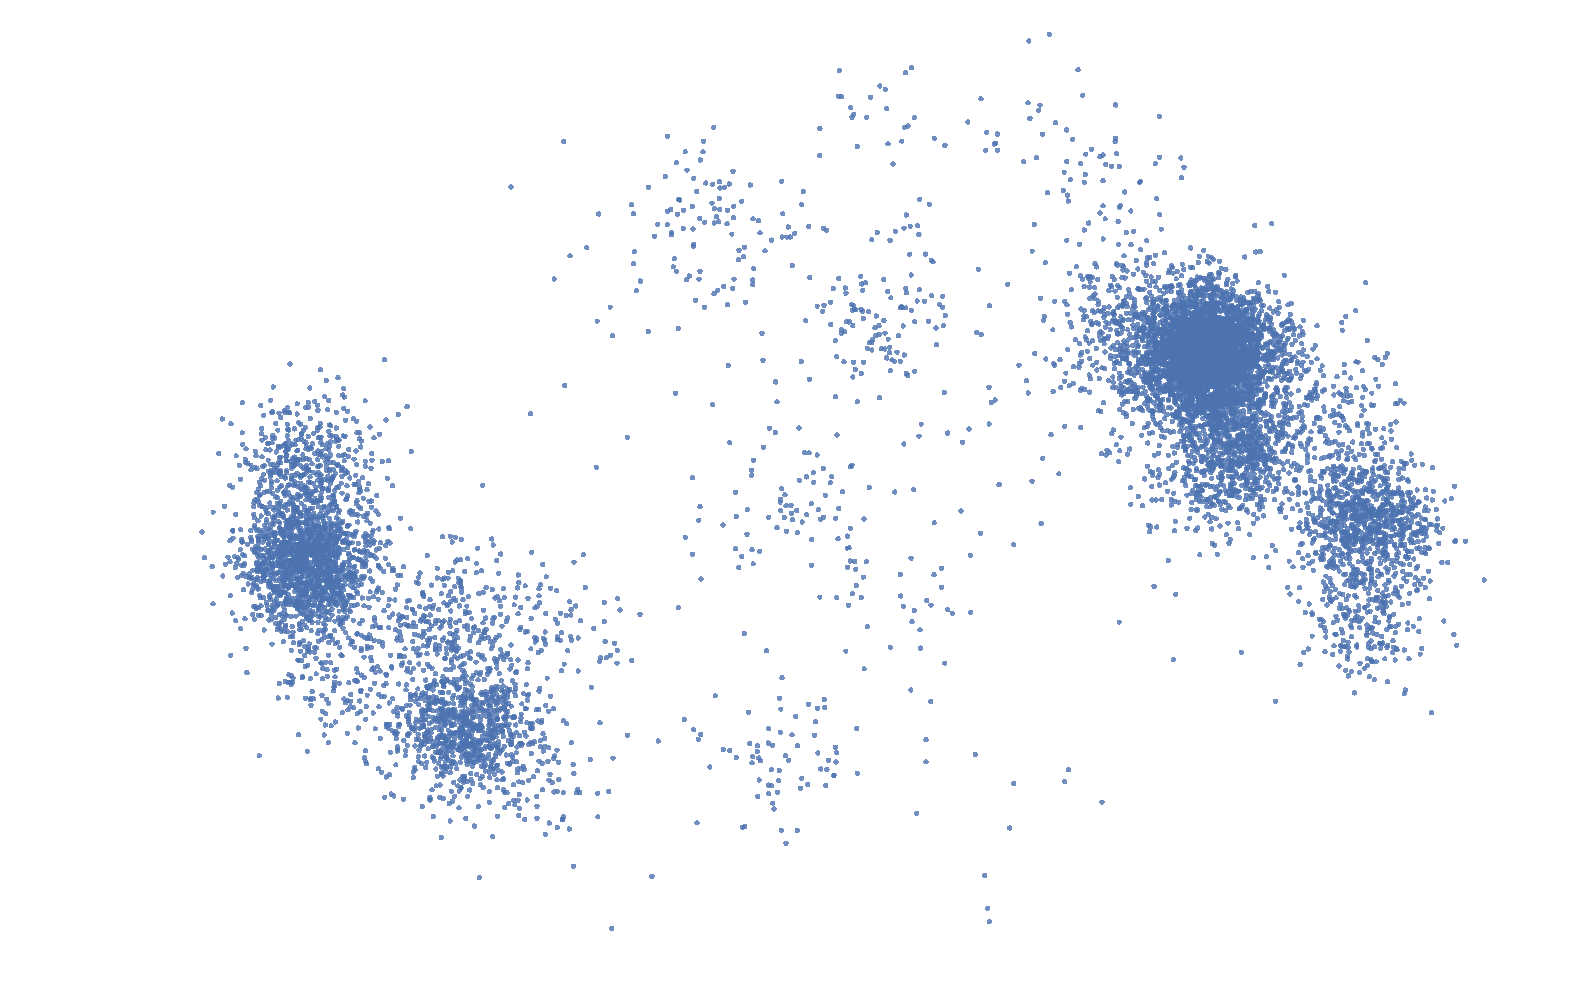
\includegraphics[width=0.8\textwidth]{images/continuous-tempering/boltzmann-machine-relaxation-samples-cropped}
\caption[Boltzmann machine relaxation samples.]{Two-dimensional projection of 10\,000 independent samples from a Gaussian mixture relaxation of a Boltzmann machine distribution. The parameters $\mtx{W}$ and $\vct{b}$ of the Boltzmann machine distribution were generated as described in the main text, with here $D_B = 28$ (rather than $D_B = 30$ as in the experiments) as independent sampling from larger systems exceeded the memory available on the workstation used. The two components shown correspond to the two eigenvectors of the generated basis $\mtx{R}$ with the largest corresponding eigenvalues.}
\label{fig:bmr-samples-2d}
\end{figure}

A Gaussian base distribution and approximate normalising constant $\zeta$ were fitted to each the 10 relaxation target densities by matching moments to a mixture of variational Gaussian approximations (individually fitted using a mean-field approach based on the underlying Boltzmann machine distribution) as described in Section \ref{sec:choosing-base-density}. All methods used the same base distribution and $\zeta$ was used to set the prior on the inverse temperatures in all methods (equivalent to $w_k = -\beta_k\zeta$ in the earlier description of \ac{ST}).

For \ac{ST}, a \emph{Rao Blackwellised} estimate of the normalising constant $\normconst$ was used as described in \citep{carlson2016partition} and an estimator equivalent to \eqref{eq:ct-target-expc-estimator} used to allow estimation of the moments from all of the samples rather than just those for which $\rvar{k}=K$ (with our estimator found to always give better results than the standard \ac{ST} estimator in these experiments). For each of \ac{ST}, Gibbs \ac{CT} and \ac{AIS} for the updates to the target variables $\rvct{x}$ given a fixed inverse temperature (index in the case of \ac{ST}), a \ac{HMC} transition operator (Algorithm \ref{alg:hamiltonian-monte-carlo}) was used with $\delta t = 0.5$, $L = 20$. For \ac{ST} the inverse temperature values used a sigmoidal spacing
\begin{equation}\label{eq:sigmoidal-beta-schedule}
  \tilde{\beta}_k = \lpa 1 + \exp\lpa -4\frac{2k-K}{K}\rpa\rpa^{-1} ~~\forall k \in \lbrace 0\,...\,K \rbrace, \quad
  \beta_k = \frac{\tilde{\beta}_k - \tilde{\beta}_0}{\tilde{\beta}_K - \tilde{\beta}_0}
\end{equation}
with $K=1000$ used based on initial pilot runs, and independent multinomial resampling from $\prob{\rvar{k}|\rvct{x}}$ for the updates to the temperature index. For \ac{AIS} separate runs with $K=1000$, $K=5000$ and $K=10000$ inverse temperature $\beta_k$ values were used to obtain estimates at different run times, using the same sigmoidal spacing \eqref{eq:sigmoidal-beta-schedule} as for \ac{ST} and the estimate for each $K$ based on $N=100$ \ac{AIS} independent runs to produce $N$ importance samples. For the \ac{CT-HMC} chains a \ac{HMC} transition operator with $\delta t=0.5$ and $L=20$ was used with the mass value for the temperature control variable set to $m=1$.

\begin{figure}
\centering
\begin{subfigure}[b]{.7\linewidth}
\vskip 0pt
\centering
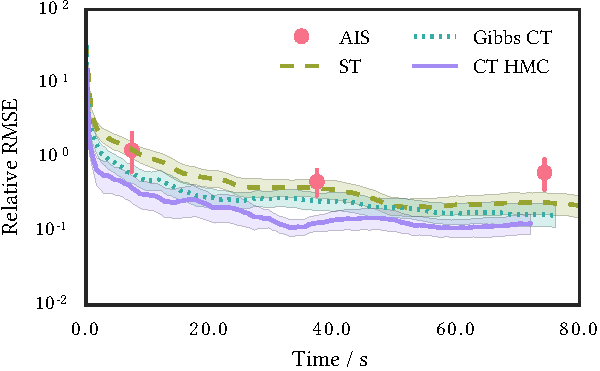
\includegraphics[width=0.95\textwidth]{images/continuous-tempering/gaussian-bm-relaxation-30-unit-scale-6-log-norm-rmses} 
\caption{$\log \normconst$}\label{sfig:bmr-30-unit-scale-6-log-norm}
\end{subfigure}
\\[5mm]
\begin{subfigure}[b]{.7\linewidth}
\vskip 0pt
\centering
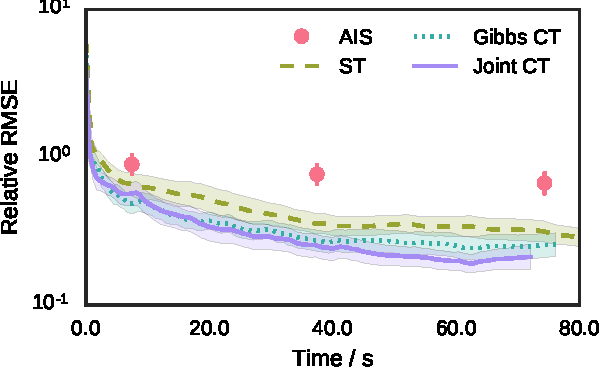
\includegraphics[width=0.95\textwidth]{images/continuous-tempering/gaussian-bm-relaxation-30-unit-scale-6-mean-rmses}
\caption{$\expc{\rvct{x}}$}\label{sfig:bmr-30-unit-scale-6-mean}
\end{subfigure}
\\[5mm]
\begin{subfigure}[b]{.7\linewidth}
\vskip 0pt
\centering
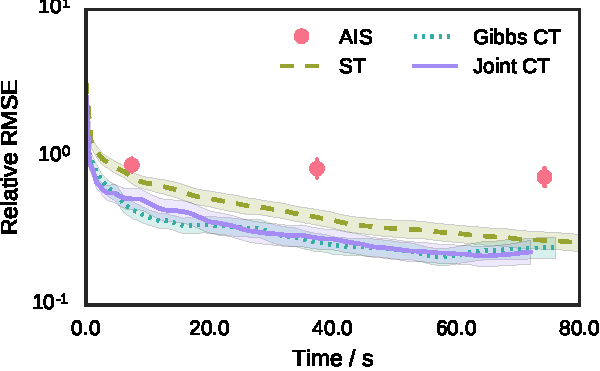
\includegraphics[width=0.95\textwidth]{images/continuous-tempering/gaussian-bm-relaxation-30-unit-scale-6-covariance-rmses} 
\caption{$\expc{\rvct{x}\rvct{x}\tr} - \expc{\rvct{x}}\expc{\rvct{x}}\tr$}\label{sfig:bmr-30-unit-scale-6-covar}
\end{subfigure}
\caption[Boltzmann machine relaxation results.]{\acp{RMSE} in empirical moments estimated from \ac{MCMC} samples against run time for various thermodynamic ensemble \ac{MCMC} methods run on Gaussian Boltzmann machine relaxation target distributions. All \acp{RMSE} are relative to the \ac{RMSE} of the corresponding approximate moments calculated using the moment-matched variational mixtures, so values below $1$ represent improvement on deterministic approximation. For \ac{AIS} points across time axis represent increasing number of inverse temperatures: $(1,\, 5,\,10)\times 10^3$. For \ac{ST}, Gibbs \ac{CT} and \ac{CT-HMC} curves show \acp{RMSE} for expectations calculated with increasing number of samples from chains. All curves / points show mean across 10 runs for each of 10 generated parameter sets. Filled regions / error bars show $\pm 3$ standard errors of mean.}
\label{fig:bmr-30-unit-scale-6-results}
\end{figure}

Plots showing the \ac{RMSE} in estimates of $\log Z$ and the mean and covariance of the relaxation distribution against computational run time for different sampling methods are shown in Figure \ref{fig:bmr-30-unit-scale-6-results}. The \ac{RMSE} values are normalised by the \ac{RMSE}s of the corresponding estimated moments used in the base density (and $\log\zeta$) such that values below unity indicate an improvement in accuracy over the variational approximation. The curves shown are \ac{RMSE}s averaged over 10 independent chains (or set of runs for \ac{AIS}) for each of the 10 generated parameter sets, with the filled regions indicating $\pm 3$ standard errors of the mean. All methods used a shared Theano \citep{theano2016theano} implementation running on a Intel Core i5-2400 quad-core CPU for the \ac{HMC} updates and so run times are roughly comparable.

The two \ac{CT} approaches, Gibbs \ac{CT} and \ac{CT-HMC}, both dominate in terms of having lower average \ac{RMSE} in all three moment estimates across all run times, with \ac{CT-HMC} showing slightly better performance on estimates of $\log\normconst$ and $\expc{\rvct{x}}$ than Gibbs \ac{CT}. The tempering approaches seem to outperform \ac{AIS} here, possibly as the highly multimodal nature of the target densities favours the ability of tempered dynamics to move the inverse temperature both up and down and so in and out of modes in the target density, unlike \ac{AIS} where the fixed sequence of temperature updates are more likely to end up with chains confined to a single mode after the initial transitions for low $\beta_k$.

\subsection{Generative image models}\label{subsec:exp-iwae}

For the next experiments, we compared the efficiency of our \ac{CT-HMC} and Gibbs \ac{CT} approaches to \ac{ST} and \ac{AIS} for marginal likelihood estimation in decoder-based generative models for images. Use of \ac{AIS} in this context was recently proposed in \citep{wu2016quantitative}. Specifically we estimate the joint marginal likelihood of 1000 generated binary images under the Bernoulli decoder distribution of two \ac{IWAE} \citep{burda2016importance} models. Each \ac{IWAE} has one stochastic hidden layer and a 50-dimensional latent space, with the two models trained on binarised versions of the MNIST \citep{lecun1998gradient} and Omniglot \citep{lake2015human} datasets using the code at \url{https://github.com/yburda/iwae}. The generated images used are shown in Figure \ref{fig:iwae-generated-test-images}.

\begin{figure}
\begin{subfigure}[b]{0.95\linewidth}
\centering
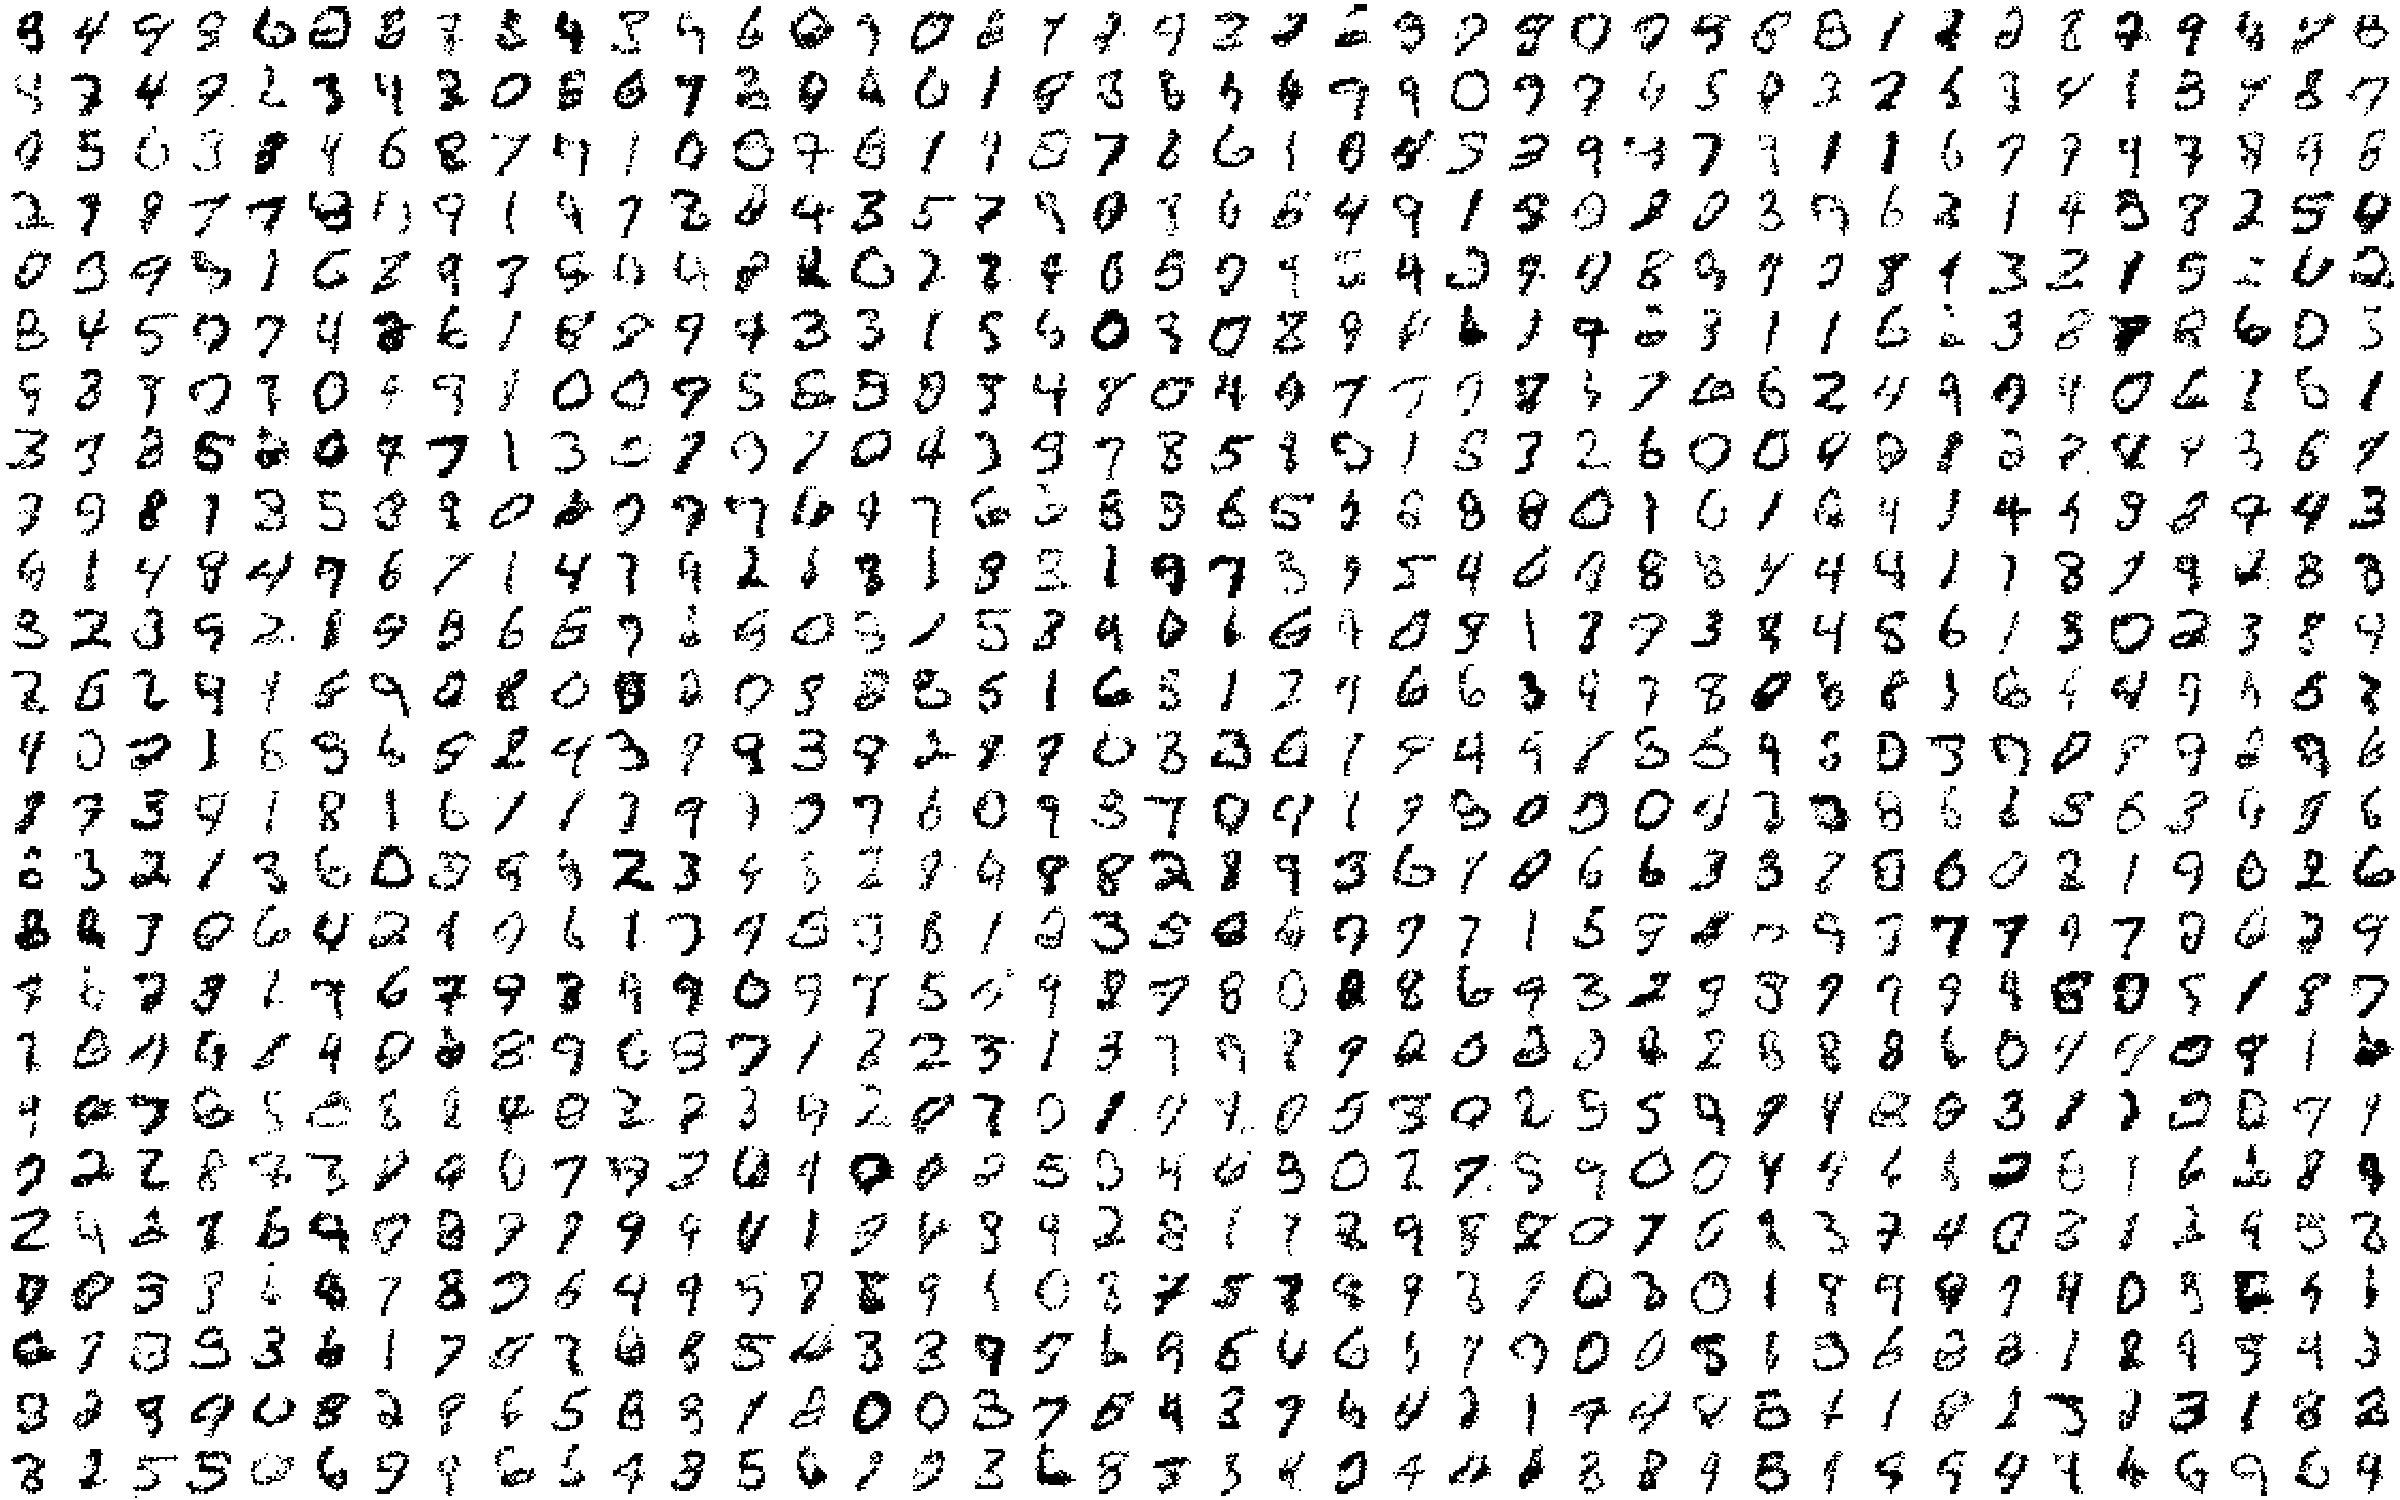
\includegraphics[width=\textwidth]{images/continuous-tempering/mnist-samples.pdf}
\caption{Generated MNIST test images.}
\label{sfig:mnist-samples}
\end{subfigure}
\\[5mm]
\begin{subfigure}[b]{0.95\linewidth}
\centering
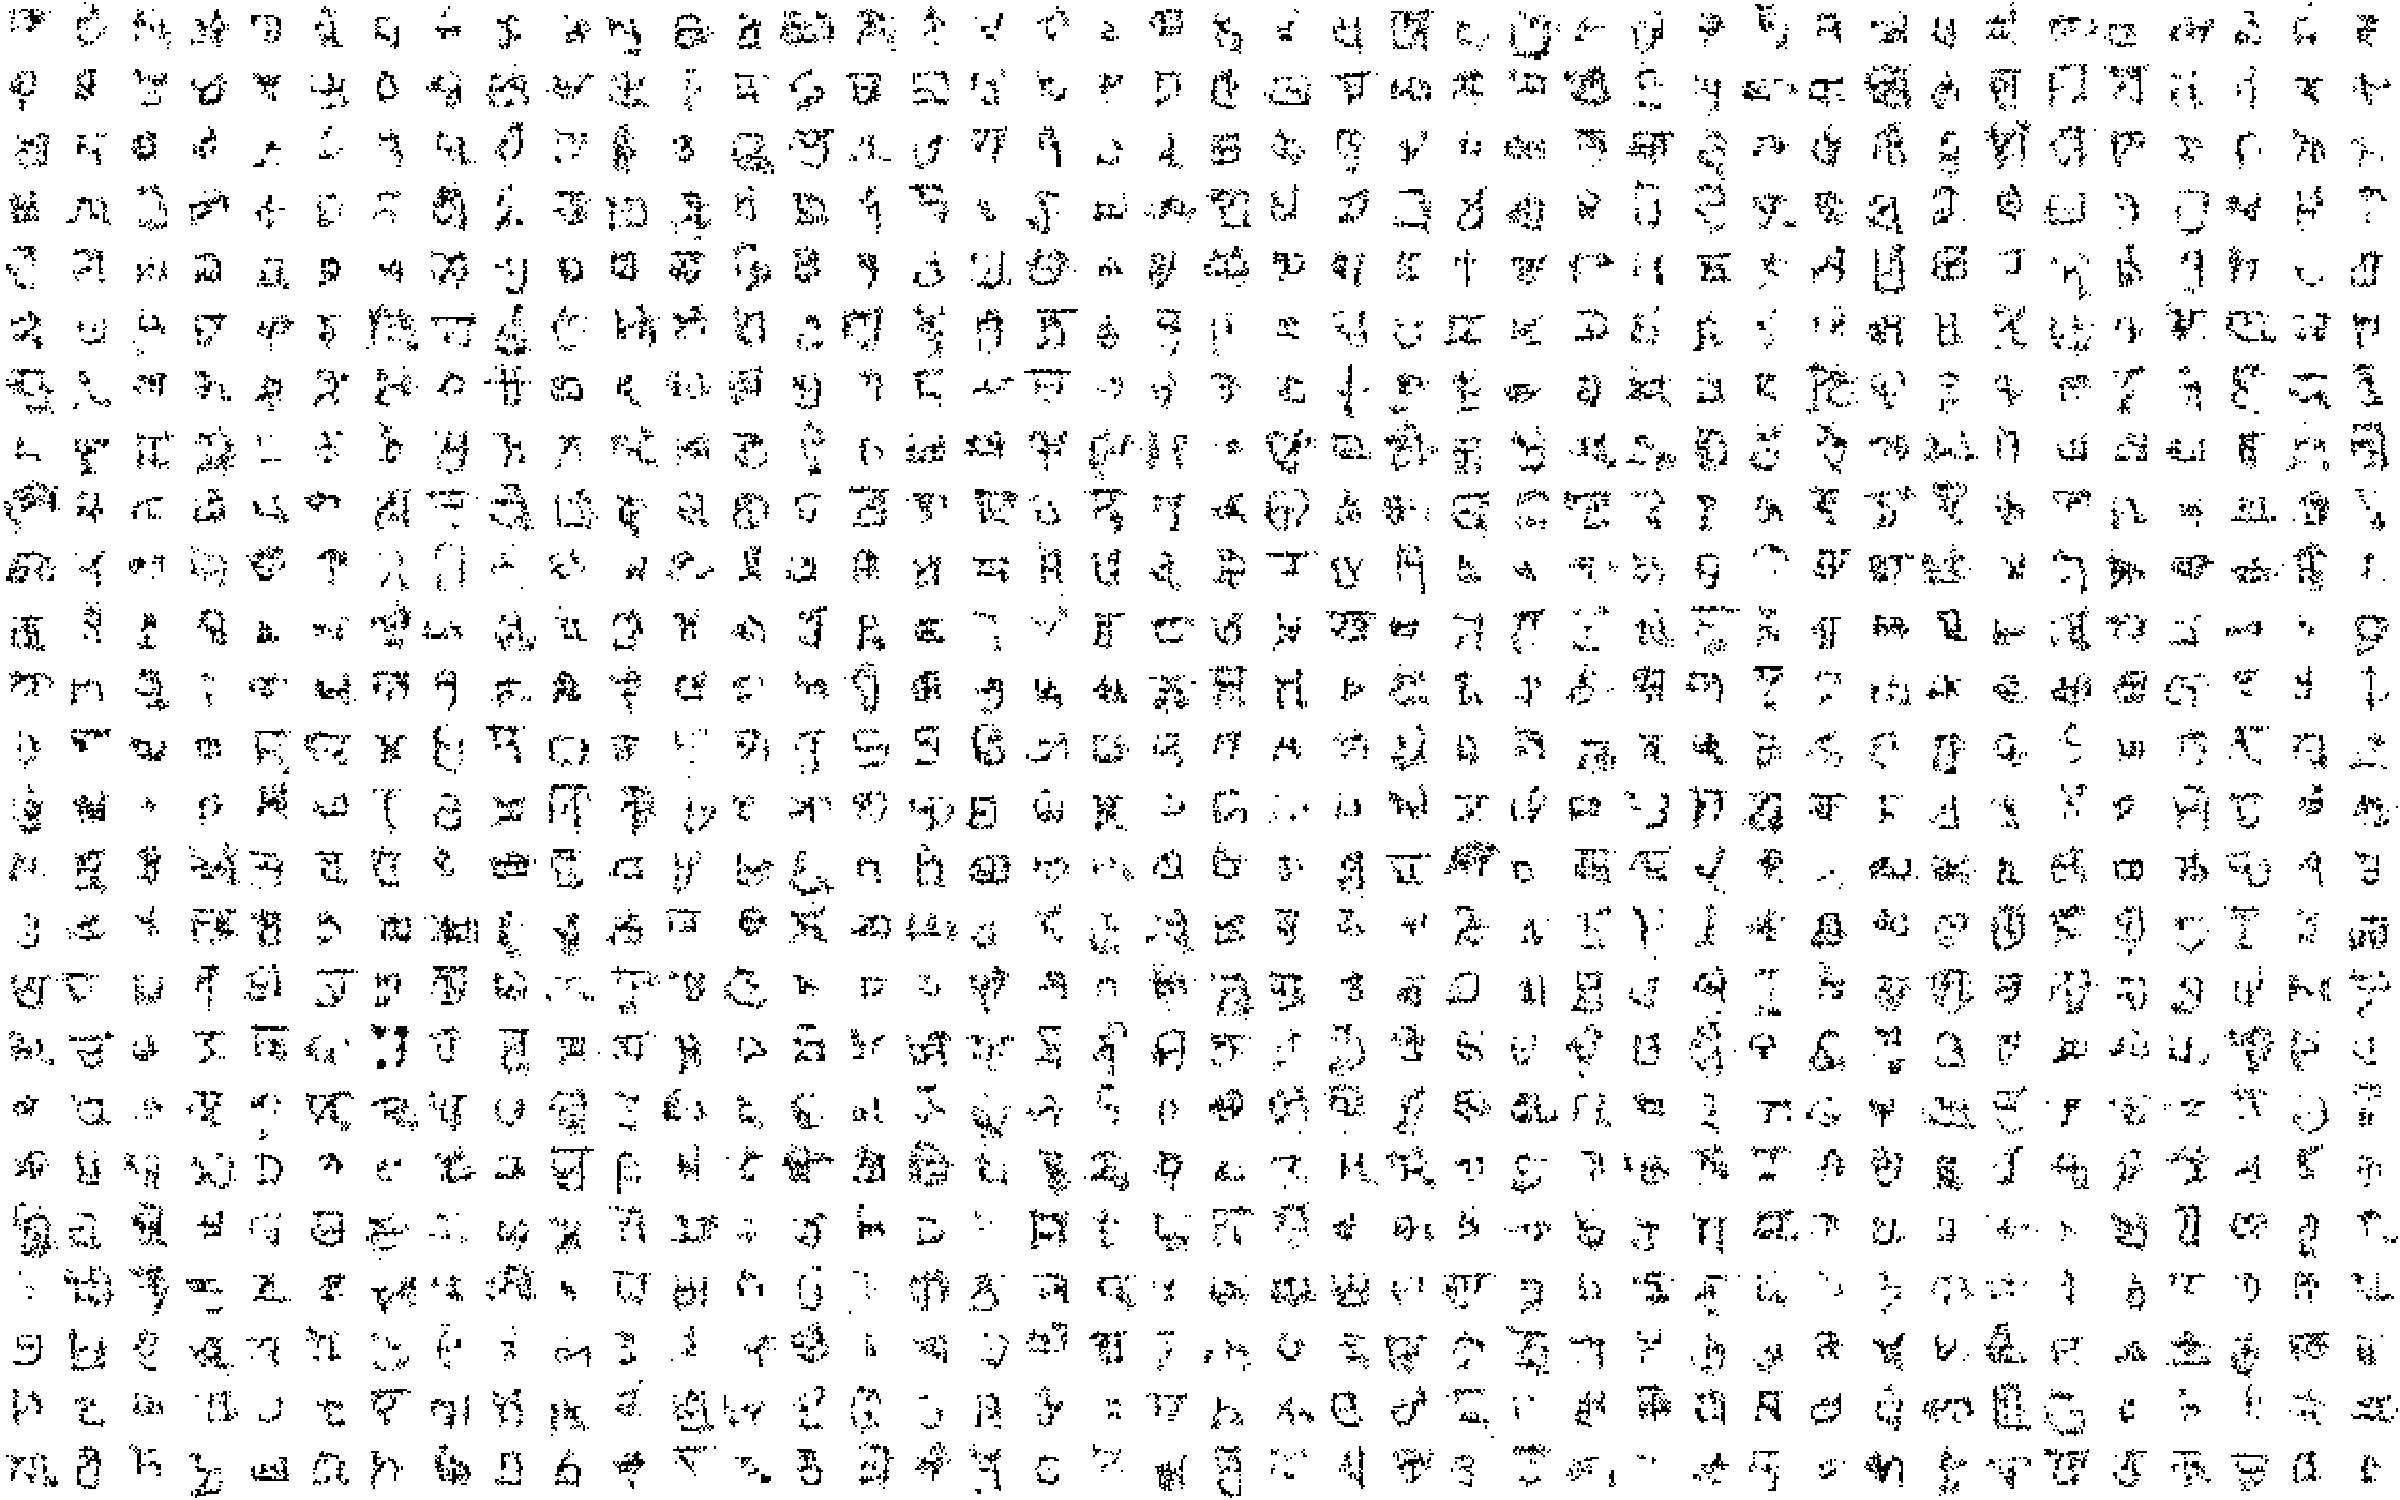
\includegraphics[width=\textwidth]{images/continuous-tempering/omniglot-samples.pdf}
\caption{Generated Omniglot test images.}
\label{sfig:omni-samples}
\end{subfigure}
\caption[\acs{IWAE} generated image datasets.]{Generated image datasets from \ac{IWAE} models that were used as the observed data for marginal likelihood estimates.}
\label{fig:iwae-generated-test-images}
\end{figure}

By performing inference on the per-image posterior densities on the latent representation given image, the joint marginal likelihood of the images can be estimated as the product of estimates of the normalising constants of the individual latent posterior densities. The use of generated images allows \ac{BDMC} \citep{grosse2015sandwiching} to be used to stochastically bound the marginal likelihood as described in Section \ref{sec:annealed-importance-sampling} with stochastic upper and lower bounds formed with long forward and backward \ac{AIS} runs (averages over 16 independent runs with 10\,000 inverse temperatures as used in \citep{wu2016quantitative}). 

As the per-image latent representations are conditionally independent given the images, chains on all the posterior densities can be run in parallel, with the experiments in this section run on a NVIDIA Tesla K40 \ac{GPU} to exploit this inherent parallelism. The encoder of the trained \ac{IWAE} models is an inference network which outputs the mean and diagonal covariance of a Gaussian variational approximation to the posterior density on the latent representation given an image and so was used to define per-image Gaussian base densities as suggested in \citep{wu2016quantitative}. Similarly the per-image $\log \zeta$ values were set using variational lower bound estimates for the per-image marginal likelihoods.

\begin{figure}
\centering
\begin{subfigure}[t]{\linewidth}
\vskip 0pt
\centering
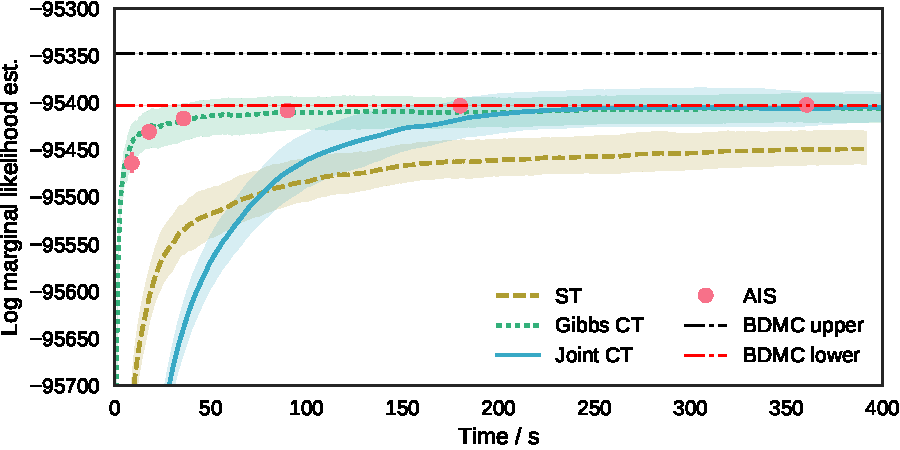
\includegraphics[width=0.95\textwidth]{images/continuous-tempering/mnist-marginal-likelihood-est}
\caption{MNIST log marginal likelihood estimates.}\label{sfig:mnist-log-marg-lik}
\end{subfigure}%
\vspace{5mm}
\begin{subfigure}[t]{\linewidth}
\vskip 0pt
\centering
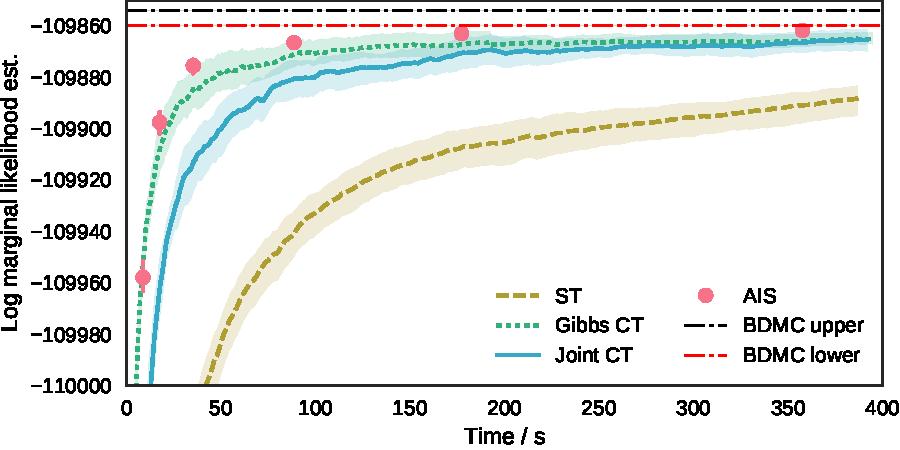
\includegraphics[width=0.95\textwidth]{images/continuous-tempering/omni-marginal-likelihood-est}
\caption{Omniglot log marginal likelihood estimates.}\label{sfig:omni-log-marg-lik}
\vskip 0pt
\end{subfigure}
\caption[\acs{IWAE} marginal likelihood estimates.]{Estimates of the log joint marginal likelihood of 1000 generated images under the Bernoulli decoder distributions of two \ac{IWAE} models trained on the MNIST and Omniglot datasets against computation time. The black / red dashed lines show stochastic upper / lower bounds calculated using long \ac{BDMC} runs. For \ac{AIS} points across time axis represent increasing number of inverse temperatures: $(50,\,100,\,200,\,500,\,1000,\,2000)$. For \ac{ST}, Gibbs \ac{CT} and joint \ac{CT} curves show estimates calculated with an increasing number of samples from chains. All curves / points show mean across 10 runs. Filled regions / error bars show $\pm 3$ standard errors of mean.
}
\label{fig:iwae-marginal-likelihood-results}
\end{figure}

The results are shown in Figure \ref{fig:iwae-marginal-likelihood-results}, with the curves / points showing average results across 10 independent runs and filled regions / bars $\pm 3$ standard error of means for the estimates. Here Gibbs \ac{CT} and \ac{AIS} perform similarly, with \ac{CT-HMC} converging less quickly and simulated tempering significantly less efficient. The quick convergence of \ac{AIS} and Gibbs \ac{CT} here suggests the posterior densities are relatively easy for the dynamics to explore and well matched by the Gaussian base densities, limiting the gains from any more coherent exploration of the extended space by the \ac{CT-HMC} updates. The higher per-leapfrog-step costs of the \ac{HMC} updates in the extended space therefore mean the \ac{CT-HMC} approach is less efficient overall here. The poorer performance of simulated tempering here is in part due to the generation of the discrete random indices becoming a bottleneck in the \ac{GPU} implementation.

A possible partial reason for the better relative performance of \ac{AIS} here compared to the experiments in Section \ref{subsec:exp-bm-relaxations} is its more effective utilisation of the parallel compute cores available when running for example on a \ac{GPU}. Multiple \ac{AIS} chains can be run for each data point and then the resulting unbiased estimates for each data points marginal likelihood averaged (reducing the per data point variance) before taking their product for the joint marginal likelihood estimate. While it is also possible to run multiple tempered chains per data point and similarly combine the estimates, empirically we found that greater gains in estimation accuracy came from running a single longer chain rather than multiple shorter chains of total length equivalent to the longer chain. This can be explained by the initial warm-up transients of each shorter chain having a greater biasing effect on the overall estimate compared to running longer chains. Therefore an increase in the number of parallel compute cores available seems to give greater gains for \ac{AIS} versus the tempering methods.

\subsection{Hierarchical regression model}\label{subsec:exp-hier-regression}

\begin{figure}
\centering
\includetikz{radon-hierarchical-linear-regression-factor-graph}
\caption{Radon hierarchical regression model.}
\label{sfig:hier-lin-regression-factor}
\end{figure}%

\begin{figure}
\centering
\vskip 0pt
\centering
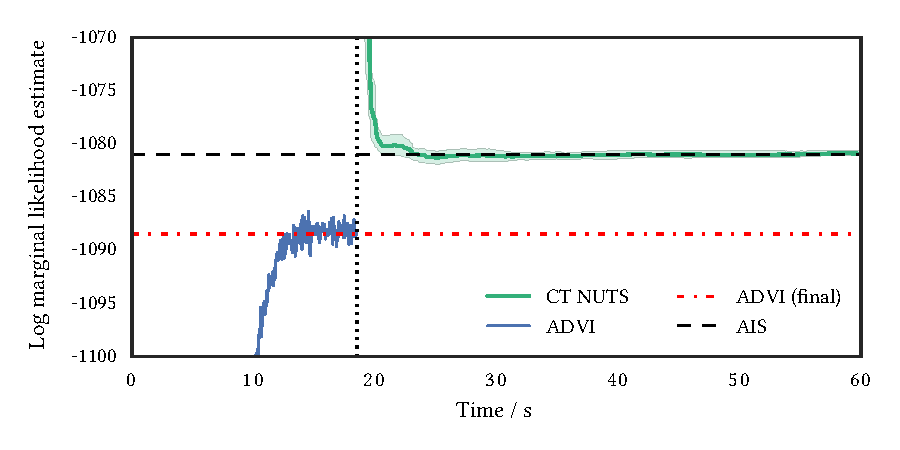
\includegraphics[width=0.9\textwidth]{images/continuous-tempering/hier-lin-regression-marg-lik}
\vskip 0pt
\caption[Radon model marginal likelihood estimates.]{Log marginal likelihood estimates against run time for hierarchical regression model. Black dashed line shows estimated log marginal likelihood from a long \ac{AIS} run which is used as a proxy ground truth. The noisy blue curve shows the \emph{evidence lower bound} \ac{ADVI} objective over training and the red dot-dashed line the final converged value used for $\log\zeta$. The green curve shows log marginal likelihood estimates using samples from \ac{NUTS} chains running on the extended joint density in the estimator \eqref{eq:ct-norm-const-estimator}, with the run time corresponding to increasing samples being included in the estimator (offset by initial \ac{ADVI} run time). Curve shows mean over 10 runs and filled region $\pm 3$ standard errors of mean.}
\label{fig:hier-lin-regression}
\end{figure}

As a final experiment, we apply our \ac{CT-HMC} approach to perform inference in a hierarchical regression model for predicting indoor radon measurements \citep{gelman2006data}. To illustrate the ease of integrating our approach in existing \ac{HMC}-based inference software, this experiment was performed with the Python package PyMC3 \citep{salvatier2016probabilistic}, with its \ac{ADVI} feature used to fit the base density and its implementation of the adaptive
\ac{NUTS} \citep{hoffman2014no} \ac{HMC} variant used to sample from the extended space.

The regression target in the dataset is measurements of the amount of radon gas $\rvar{y}^{(i)}$ in $N=919$ households. Two continuous regressors $\vct{x}^{(i)}$ and one categorical regressor $c^{(i)}$ are provided per household. A multilevel regression model defined by the factor graph in \ref{sfig:hier-lin-regression-factor} was used. The model includes five scalar parameters $(\upsigma_{\rvct{a}},\,\upmu_{\rvct{a}},\,\upsigma_{\rvct{b}},\,\upmu_{\rvct{b}},\,\upepsilon)$, an 85-dimensional intercept vector $\rvct{a}$ and a two-dimensional regressor coefficients vector $\rvct{b}$, giving 92 parameters in total. As an example task, we consider inferring the marginal likelihood of the data under the model. %Estimation of the marginal likelihood from \ac{MCMC} samples of the target density alone is non-trivial, with approaches such as the harmonic mean estimator having high variance. Here we try to establish if our approach can be used in a black-box fashion to compute a reasonable estimate of the marginal likelihood.

As our `ground truth' we use a large batch of long \ac{AIS} runs (average across 100 runs of 10000 inverse temperatures) on a separate Theano implementation of the model. We use \ac{ADVI} to fit a diagonal covariance Gaussian variational approximation to the target density and use this as the base density. \ac{NUTS} chains, initialised at samples from the base density, were then run on the extended space for 2500 iterations. The samples from these chain were used to compute estimates of the normalising constant (marginal likelihood) using the estimator \eqref{eq:ct-norm-const-estimator}. The results are shown in Figure \ref{fig:hier-lin-regression}. It can be seen that estimates from the \ac{NUTS} chains in the extended continuously tempered space quickly converge to a marginal likelihood estimate very close to the \ac{AIS} estimate, and significantly improve over the final lower bound on the marginal likelihood that \ac{ADVI} converges to.

\section{Discussion}

The continuous tempering approaches we have proposed in this chapter are a simple but powerful extension to existing simulated tempering methods which can both help exploration of distributions with multiple isolated modes and allow estimation of the normalisation constant of the target distribution. We propose a novel importance sampling inspired method for using all of a tempered chains samples to estimate expectations with respect to the target distribution, overcoming the wastefulness of the standard estimator typically used in simulated tempering which computes estimates using only subsets of states. The use of this estimator also means that we can use a continuous inverse temperature formulation that reduces the number of free parameters the user needs to tune by removing the need to choose a set of discrete inverse temperatures.

A key advantage of the \ac{CT-HMC} method is its ease of implementation - it simply requires running \ac{HMC} in an extended state space and so can easily be used for example within existing probabilistic programming software such as PyMC3 \citep{salvatier2016probabilistic} and Stan \citep{carpenter2016stan} as seen in the last experiment in Section \ref{sec:ct-experiments}. By updating the temperature jointly with the original target state, it is also possible to leverage adaptive \ac{HMC} variants such as \ac{NUTS} \citep{hoffman2014no} to perform tempered inference in a `black-box' manner without the need to separately tune the updates of the inverse temperature variable.

The Gibbs \ac{CT} method also provides a relatively black-box framework for tempering. Compared to \ac{ST} it removes the need to choose the number and spacing of discrete inverse temperatures and also replaces generation of a discrete random variate from a categorical distribution when updating $\upbeta$ given $\rvct{x}$ (which as seen in Section \ref{subsec:exp-iwae} can become a computational bottleneck) with generation of a truncated exponential variate (which can be performed efficiently by inverse transform sampling). Compared to the \ac{CT-HMC} approach, the Gibbs approach is less simple to integrate in to existing \ac{HMC} code due to the separate $\upbeta$ updates, but eliminates the need to tune the temperature control mass value $m$ and achieved similar or better sampling efficiency in the experiments in Section \ref{sec:ct-experiments}.

In models we considered in experiments, the sampling efficiency using the proposed continuous tempering approaches was always as good or better than simulated tempering. The comparison with \ac{AIS} was less clear cut with the continuous tempering approaches outperforming \ac{AIS} in the Boltzmann machine relaxation experiments but \ac{AIS} generally doing better in the generative image model experiments (though Gibbs \ac{CT} was competitive). The tempering approaches and \ac{AIS} are less directly comparable due to the different basic inference approach being used to compute expectations --- importance sampling with independent proposals --- versus the Markov chain approaches of the tempering methods. This for example gave different tradeoffs in the utilisation of parallel compute, with it generally simpler to efficiently exploit more parallelism in \ac{AIS}. Our proposed use of an importance sampling estimator with samples generated using a Markov chain does bear some interesting similarities with \ac{AIS}, however the approaches remain quite different, with \ac{AIS} using a Markov chain to construct each independent proposal rather than to sample from the proposal distribution, and the \ac{AIS} normalising constant estimate is unbiased unlike the consistent estimator of our approach.

Our proposal to use variational approximations to select the base distribution helps improve the ability to scale tempering methods to complex high-dimensional target distributions were simple uninformative base distributions can lead to poor performance. Approaches such as \ac{ADVI} \citep{kucukelbir2016automatic} can be applied to a wide range of models with differentiable densities with minimal need for user input and efficient implementations are available in frameworks such as Stan and PyMC3. 

Our use of variational inference  within an \ac{MCMC} framework can be viewed within the context of several existing approaches which suggest combining variational and \ac{MCMC} inference methods. \emph{Variational MCMC} \citep{de2001variational} proposes using a variational approximation as the basis for a proposal distribution in a Metropolis-Hastings \ac{MCMC} method. \emph{MCMC and Variational Inference: Bridging the Gap} \citep{salimans2015markov} includes parametrised \ac{MCMC} transitions within a (stochastic) variational approximation and optimises the variational bound over these (and a base distribution's) parameters. Here we exploit cheap but biased variational approximations to a target distribution and its normalising constant, and use them within an \ac{MCMC} method which gives asymptotically exact results to help improve sampling efficiency.